%%% The main file. It contains definitions of basic parameters and includes all other parts.

%% Settings for single-side (simplex) printing
% Margins: left 40mm, right 25mm, top and bottom 25mm
% (but beware, LaTeX adds 1in implicitly)
\documentclass[12pt,a4paper]{report}
\setlength\textwidth{145mm}
\setlength\textheight{247mm}
\setlength\oddsidemargin{15mm}
\setlength\evensidemargin{15mm}
\setlength\topmargin{0mm}
\setlength\headsep{0mm}
\setlength\headheight{0mm}
% \openright makes the following text appear on a right-hand page
\let\openright=\clearpage

%% Settings for two-sided (duplex) printing
% \documentclass[12pt,a4paper,twoside,openright]{report}
% \setlength\textwidth{145mm}
% \setlength\textheight{247mm}
% \setlength\oddsidemargin{14.2mm}
% \setlength\evensidemargin{0mm}
% \setlength\topmargin{0mm}
% \setlength\headsep{0mm}
% \setlength\headheight{0mm}
% \let\openright=\cleardoublepage

%% Generate PDF/A-2u
\usepackage[a-2u]{pdfx}

%% Character encoding: usually latin2, cp1250 or utf8:
\usepackage[utf8]{inputenc}

%% Prefer Latin Modern fonts
\usepackage{lmodern}

%% Further useful packages (included in most LaTeX distributions)
\usepackage{amsmath}        % extensions for typesetting of math
\usepackage{amsfonts}       % math fonts
\usepackage{amsthm}         % theorems, definitions, etc.
\usepackage{bbding}         % various symbols (squares, asterisks, scissors, ...)
\usepackage{bm}             % boldface symbols (\bm)
\usepackage{graphicx}       % embedding of pictures
\usepackage{fancyvrb}       % improved verbatim environment
\usepackage{natbib}         % citation style AUTHOR (YEAR), or AUTHOR [NUMBER]
\usepackage[nottoc]{tocbibind} % makes sure that bibliography and the lists
			    % of figures/tables are included in the table
			    % of contents
\usepackage{dcolumn}        % improved alignment of table columns
\usepackage{booktabs}       % improved horizontal lines in tables
\usepackage{paralist}       % improved enumerate and itemize
\usepackage{xcolor}         % typesetting in color
\usepackage{enumitem}       % description with \item
\usepackage[colorinlistoftodos]{todonotes}
\usepackage{pifont}         % tick, cross and triangle symbols
\usepackage{epigraph}       % quote of Tim Berners-Lee

%%% Basic information on the thesis

% Thesis title in English (exactly as in the formal assignment)
\def\ThesisTitle{Dietary profile and customized menus using Solid}

% Author of the thesis
\def\ThesisAuthor{Bc. Jiří Resler}

% Year when the thesis is submitted
\def\YearSubmitted{2024}

% Name of the department or institute, where the work was officially assigned
% (according to the Organizational Structure of MFF UK in English,
% or a full name of a department outside MFF)
\def\Department{Department of Software Engineering}

% Is it a department (katedra), or an institute (ústav)?
\def\DeptType{Department}

% Thesis supervisor: name, surname and titles
\def\Supervisor{RNDr. Jakub Klímek, Ph.D.}

% Supervisor's department (again according to Organizational structure of MFF)
\def\SupervisorsDepartment{Department of Software Engineering}

% Study programme and specialization
\def\StudyProgramme{Software and Data Engineering}
\def\StudyBranch{Software engineering}

% An optional dedication: you can thank whomever you wish (your supervisor,
% consultant, a person who lent the software, etc.)
\def\Dedication{%
Dedication.
}

% Abstract (recommended length around 80-200 words; this is not a copy of your thesis assignment!)
\def\Abstract{%
Abstract.
}

% 3 to 5 keywords (recommended), each enclosed in curly braces
\def\Keywords{%
{solid}, {data}, {linked data}, {RDF}, {redecentralization of web}, {read write web}, {diet}, {food}
}

%% The hyperref package for clickable links in PDF and also for storing
%% metadata to PDF (including the table of contents).
%% Most settings are pre-set by the pdfx package.
\hypersetup{unicode}
\hypersetup{breaklinks=true}

% Definitions of macros (see description inside)
%%% This file contains definitions of various useful macros and environments %%%
%%% Please add more macros here instead of cluttering other files with them. %%%

%%% Minor tweaks of style

% These macros employ a little dirty trick to convince LaTeX to typeset
% chapter headings sanely, without lots of empty space above them.
% Feel free to ignore.
\makeatletter
\def\@makechapterhead#1{
  {\parindent \z@ \raggedright \normalfont
   \Huge\bfseries \thechapter. #1
   \par\nobreak
   \vskip 20\p@
}}
\def\@makeschapterhead#1{
  {\parindent \z@ \raggedright \normalfont
   \Huge\bfseries #1
   \par\nobreak
   \vskip 20\p@
}}
\makeatother

% This macro defines a chapter, which is not numbered, but is included
% in the table of contents.
\def\chapwithtoc#1{
\chapter*{#1}
\addcontentsline{toc}{chapter}{#1}
}

% Draw black "slugs" whenever a line overflows, so that we can spot it easily.
\overfullrule=1mm

%%% Macros for definitions, theorems, claims, examples, ... (requires amsthm package)

\theoremstyle{plain}
\newtheorem{thm}{Theorem}
\newtheorem{lemma}[thm]{Lemma}
\newtheorem{claim}[thm]{Claim}

\theoremstyle{plain}
\newtheorem{defn}{Definition}

\theoremstyle{remark}
\newtheorem*{cor}{Corollary}
\newtheorem*{rem}{Remark}
\newtheorem*{example}{Example}

%%% An environment for proofs

\newenvironment{myproof}{
  \par\medskip\noindent
  \textit{Proof}.
}{
\newline
\rightline{$\qedsymbol$}
}

%%% An environment for typesetting of program code and input/output
%%% of programs. (Requires the fancyvrb package -- fancy verbatim.)

\DefineVerbatimEnvironment{code}{Verbatim}{fontsize=\small, frame=single}

%%% The field of all real and natural numbers
\newcommand{\R}{\mathbb{R}}
\newcommand{\N}{\mathbb{N}}

%%% Useful operators for statistics and probability
\DeclareMathOperator{\pr}{\textsf{P}}
\DeclareMathOperator{\E}{\textsf{E}\,}
\DeclareMathOperator{\var}{\textrm{var}}
\DeclareMathOperator{\sd}{\textrm{sd}}

%%% Transposition of a vector/matrix
\newcommand{\T}[1]{#1^\top}

%%% Various math goodies
\newcommand{\goto}{\rightarrow}
\newcommand{\gotop}{\stackrel{P}{\longrightarrow}}
\newcommand{\maon}[1]{o(n^{#1})}
\newcommand{\abs}[1]{\left|{#1}\right|}
\newcommand{\dint}{\int_0^\tau\!\!\int_0^\tau}
\newcommand{\isqr}[1]{\frac{1}{\sqrt{#1}}}

%%% Various table goodies
\newcommand{\pulrad}[1]{\raisebox{1.5ex}[0pt]{#1}}
\newcommand{\mc}[1]{\multicolumn{1}{c}{#1}}


% Title page and various mandatory informational pages
\begin{document}
%%% Title page of the thesis and other mandatory pages

%%% Title page of the thesis

\pagestyle{empty}
\hypersetup{pageanchor=false}
\begin{center}

\centerline{\mbox{
\includegraphics[width=166mm]{../img/logo-en.pdf}}}

\vspace{-8mm}
\vfill

{\bf\Large MASTER THESIS}

\vfill

{\LARGE\ThesisAuthor}

\vspace{15mm}

{\LARGE\bfseries\ThesisTitle}

\vfill

\Department

\vfill

{
\centerline{\vbox{\halign{\hbox to 0.45\hsize{\hfil #}&\hskip 0.5em\parbox[t]{0.45\hsize}{\raggedright #}\cr
Supervisor of the master thesis:&\Supervisor \cr
\noalign{\vspace{2mm}}
Study programme:&\StudyProgramme \cr
\noalign{\vspace{2mm}}
Study branch:&\StudyBranch \cr
}}}}

\vfill

% Zde doplňte rok
Prague \YearSubmitted

\end{center}

\newpage

%%% Here should be a bound sheet included -- a signed copy of the "master
%%% thesis assignment". This assignment is NOT a part of the electronic
%%% version of the thesis. DO NOT SCAN.

%%% A page with a solemn declaration to the master thesis

\openright
\hypersetup{pageanchor=true}
\pagestyle{plain}
\pagenumbering{roman}
\vglue 0pt plus 1fill

\noindent
I declare that I carried out this master thesis independently, and only with the cited
sources, literature and other professional sources. It has not been used to obtain another
or the same degree.

\medskip\noindent
I understand that my work relates to the rights and obligations under the Act No.~121/2000 Sb.,
the Copyright Act, as amended, in particular the fact that the Charles
University has the right to conclude a license agreement on the use of this
work as a school work pursuant to Section 60 subsection 1 of the Copyright~Act.

\vspace{10mm}

\hbox{\hbox to 0.5\hsize{%
In \hbox to 6em{\dotfill} date \hbox to 6em{\dotfill}
\hss}\hbox to 0.5\hsize{\dotfill\quad}}
\smallskip
\hbox{\hbox to 0.5\hsize{}\hbox to 0.5\hsize{\hfil Author's signature\hfil}}

\vspace{20mm}
\newpage

%%% Dedication

\openright

\noindent
\Dedication

\newpage

%%% Mandatory information page of the thesis

\openright

\vbox to 0.5\vsize{
\setlength\parindent{0mm}
\setlength\parskip{5mm}

Title:
\ThesisTitle

Author:
\ThesisAuthor

\DeptType:
\Department

Supervisor:
\Supervisor, \SupervisorsDepartment

Abstract:
\Abstract

Keywords:
\Keywords

\vss}

\newpage

\openright
\pagestyle{plain}
\pagenumbering{arabic}
\setcounter{page}{1}


%%% A page with automatically generated table of contents of the master thesis

\tableofcontents

%%% Each chapter is kept in a separate file
\chapter*{Introduction}
\addcontentsline{toc}{chapter}{Introduction}

Health is the most important thing we have in our lives.
If we want to be healthy we need to, among other things, think about what we eat.
People today are trying various diets in order to stay in shape and feel good.
There are also many people who suffer from food allergies who need to pick carefully what they eat, as some food is harmful to them. 

If a person who is on a diet or has an allergy decides to visit a restaurant which they have never been to, they spend a lot of time reading the restaurant's menu. 
They need to browse it and read ingredients of every meal in order to find one which is healthy for them to eat.

In this thesis we will document the process of the creation of a web application whose purpose will be to help these people to be able to quickly choose what they want to eat at a restaurant. 
The application will achieve this by letting its users create their personal profile and within it to specify what allergies they have or what diets they are on. 
It will also enable restaurant providers to create menus online. 
When a visitor will browse a restaurant's menu, the application will make it possible to only display those meals which the visitor is able to eat according to their profile.

Also, we need to be aware that whether someone is on a diet or has an allergy are personal information which the user may be sensitive about.

We will therefor design and implement the application in a safe and modern way which will ensure that only the user can view and manipulate with their personal profile data.

\listoftodos
\chapter{Preliminaries}
We will start by introducing the Solid technology.
This chapter contains an explanation of terms specific to Solid which will be used throughout this thesis.

% Glossary
% EU - European Union
% Solid

% Solid pod

% WebID

% IRI

% URL

% Solid provider

% \section{Semantic Web - the Solid technology}

\chapter{Problem analysis}
Our first step is to define what should the application be able to do and also for whom it is created.
For this reason we identify user roles and their requirements. 
After that specify use cases of each user role and describe those via use case scenarios.

\section{Target group}
The application will focus on restaurants and their guests in the European Union.
The reason behind this is that the EU enforces restaurants to inform their guests about allergens contained in the food they serve, and has already established rules for how to do it.
We would like for the application to be usable internationally, so it needs to have its user interface translated into different languages.
For this purpose we will choose the English, Slovak and Czech languages with the possibility of adding more translations in the future.

\todo[inline]{Change user role restaurant to restaurant employee}

\section{User roles}
There are two types of users who will come in contact with the application.
The first type is a \textbf{restaurant}, more specifically its employee who is responsible for creating menus.
This user needs to have a basic understanding of how to use a web browser either on a computer or on a smartphone.
The application will allow restaurant employees to create menus online and will help them with specifying allergens contained in menu items.

The second type of user is a restaurant \textbf{guest}.
They, too, need to have a basic understanding of how to use a web browser either on a computer or on a smartphone.
The application will enable a restaurant guest to create a personal profile where they will specify their food preferences, including the allergies they have and the diets they are on.
When a guest will view a restaurant's menu using the application, the displayed menu will be adapted to meet the guest's profile preferences.
The application will thus make it easier for the guest to choose what they would like to order in a particular restaurant.

\newpage

\section{User requirements}
It is good practice to use language consistently throughout requirements and that is why we are going to resolve what keywords will we use and what will they mean.
If a requirement states that the application \textbf{shall} do something then it means that the requirement is mandatory for the application and has to be addressed in the design phase which follows after this chapter. 
The word \textbf{should} is used in requirements which are desired by users but are not critical for the application's usability.
Last but not least, usage of the word \textbf{must} indicates a domain constraint.
Also, we will substitute the user role restaurant for \emph{restaurant employee} where it will be more convenient.
This list of requirements is inspired by interviewing a restaurant\footnote{\url{pizzabudca.sk}  \label{fnlabel}} employee and also two former restaurant\footnote{\url{sokolzabreh.cz/hospudka}  \label{fnlabel}} owners.

\subsection{Functional requirements}
\subsubsection{Guest user role requirements}
A guest is expected to be logged in to the application if not stated otherwise in a requirement.

\begin{description}
    \item [Req. 1.1:] The application shall enable a restaurant guest to specify what allergies they have.
    \item [Req. 1.2:] The application shall enable a restaurant guest to specify what diets they are on.
    \item [Req. 1.3:] The application should enable a restaurant guest to specify what food and beverages they like and dislike.
    \todo[inline]{maybe remove this requirement as it is not testable, leave only reqs 1.5 and 1.6}
    \item [Req. 1.4:] The application shall enable a restaurant guest to view a menu of the restaurant which is personalized based on the guest's profile.

    \emph{Rationale:} A personalized menu highlights or hides items of a menu, so that a guest can quickly choose what they want to order. 
    \item [Req. 1.5:] The application shall be able to sort meals in a menu by whether a viewing guest can eat them according to their profile.
    \item [Req. 1.6:] The application shall be able to hide meals of a menu which, according to their profile, a viewing guest cannot eat.
    \item [Req. 1.7:] A guest shall be able to view a restaurant's menu by specifying the menu's IRI.
    \item [Req. 1.8:] A guest should be able to view a menu by scanning a QR code on a printed menu.

    \emph{Rationale:} The QR code will link to the URL of the application and will provide it with the IRI of the menu just like in the requirement 1.7.
    \item [Req. 1.9:] A guest should be able to specify the IRI of a restaurant and browse its menus.

    \emph{Rationale:} A restaurant can have multiple menus valid at the same time. 
    \item [Req. 1.10:] A guest shall be able to mark a restaurant as their favorite.
    
    \emph{Rationale:} The guest should have a set of their favorite restaurants which will be used for other application's functionality like the requirement 1.11.
    \item [Req. 1.11:] A guest shall be able to see an overview of currently served meals by their favorite restaurants.
    \item [Req. 1.12:] A guest should be able to filter menu items based on what diet they are part of.

    \emph{Rationale:} no matter what is in their profile
    \item [Req. 1.13:] A non-authenticated guest should have access to the application's functionalities stated in requirements 1.7, 1.8, 1.9 and 1.12. 
    
    \emph{Rationale:} None of these features require a guest to be logged in. The application should be also useful for people without a profile.
    \item [Req. 1.14:] The application should be able to translate a menu to the same language as that of the currently displayed user interface.
\end{description}

\subsubsection{Restaurant user role requirements}
\begin{description}
    \item [Req. 2.1:] A restaurant employee shall be able to create a menu for a specific day.

    \emph{Rationale:} Restaurants often have daily menus.
    \item [Req. 2.2:] A restaurant employee shall be able to create a stable menu.

    \emph{Rationale:} Most restaurants have a stable menu which is valid every day and does not change often.
    \item [Req. 2.3:] A restaurant employee should be able to create a list of beverages.

    \emph{Rationale:} Some restaurants have a separate menu for meals and for drinks.
    \item [Req. 2.4:] A restaurant employee should be able to print a menu.

    \emph{Rationale:} A printed menu can be put on tables.
    \item [Req. 2.5:] A printed menu should optionally contain a QR code which will link a guest to the application.

    \emph{Rationale:} The QR code will provide the application with the IRI of the menu.
    \item [Req. 2.6:] The application shall enable a restaurant employee to edit a previously created menu.
    \item [Req. 2.7:] The application shall enable a restaurant employee to delete a previously created menu.
    \item [Req. 2.8:] A restaurant employee should be able to set a daily menu to repeat periodically for a certain day of the week.

    \emph{Rationale:} A daily menu can be the same for a certain day of the week.
    \item [Req. 2.9:] A restaurant employee should be able to specify categories and subcategories of a menu.

    \emph{Rationale:} A menu typically consists of categories like soups, appetizers, desserts etc. These categories can have subcategories, for instance a category "Drinks" can have subcategories "Wine" and "Non-alcoholic".
    \item [Req. 2.10:] If a menu consists of categories then each menu item should be in exactly one category.
    \item [Req. 2.11:] A category in a menu should not be empty.   
    \item [Req. 2.12:] A meal in a menu should contain an ID, label, price, weight or volume, ingredients and allergens.
    \item [Req. 2.13:] A restaurant employee should be able to specify weights of ingredients contained in a meal.

    \emph{Rationale:} The weight in the requirement 2.11 is the weight of a whole meal, i.e. all ingredients' weights combined.
    \item [Req. 2.14:] A menu should optionally contain a restaurant's name, address, telephone number and opening hours.
    \item [Req. 2.15:] A restaurant employee should be able to use a previously created menu as the starting point for creating a new menu.

    \emph{Rationale:} A restaurant employee might want to create a new menu which differs only in some items of an existing menu.
    \item [Req. 2.16:] A restaurant employee should be able to specify what currency to use in a menu.
    \item [Req. 2.17:] A restaurant employee should be able to specify what weight units to use in a menu.
    \item [Req. 2.18:] A restaurant employee should be able to specify what volume units to use for liquid items in a menu.
    \item [Req. 2.19:] A restaurant employee should be able to specify what font to use in a menu.
    \item [Req. 2.20:] The application should offer at least three empty menus as templates for a restaurant employee to choose from when creating a menu.

    \emph{Rationale:} These templates can differ in what categories they have, what font they use or what currency and weight units they use.
    \item [Req. 2.21:] A restaurant employee should be able to set that a menu shall use allergen labels for displaying allergen information.

    \emph{Rationale:} Allergens can be listed within an item's description.
    \item [Req. 2.22:] A restaurant employee should be able to set that a menu shall use numbers for displaying allergen information.

    \emph{Rationale:} A menu item can contain numbers which represent allergens. This is more concise than using labels from the requirement 2.20.
    \item [Req. 2.23:] A restaurant employee should be able to set what currency, weight and volume units to use by default in a menu.
  
    \emph{Rationale:} A restaurant might use the same units in all of its menus. The purpose of this requirement is to save restaurant employees from doing repetitive work when creating menus.
    \item [Req. 2.24:] A restaurant employee should be able to share a menu on the restaurant's Facebook, Twitter and Instagram accounts.
  \end{description}

\newpage

\subsection{Non-functional requirements}
\begin{description}
    \item [Req. 3.1:] Each item of a menu must have its allergens specified.
    
    \emph{Rationale:} In the EU, there are laws\footnote{\url{data.europa.eu/eli/reg/2011/1169/2018-01-01}  \label{fnlabel}} which mandate restaurants to list allergens contained in the foods they serve.
    \item [Req. 3.2:] A menu which uses numbers for displaying allergen information must contain a legend explaining which allergen each number represents.

    \emph{Rationale:} This requirement extends the requirement 2.21.
    \item [Req. 3.3:] The application should have responsive user interface for mobile devices and desktops.
    \item [Req. 3.4:] The application should be compatible with the latest versions of all of the commonly used browsers, namely Google Chrome of version x.y, Mozilla Firefox of version x.y, Microsoft Edge of version x.y, Opera of version x.y and Safari of version x.y.
    \item [Req. 3.5:] The application shall have a user tutorial explaining its functionality for each screen defined in the design chapter.
    \item [Req. 3.6:] The application should have an English, Czech and Slovak translations.

    \emph{Rationale:} We would like for the application to be used internationally within the European Union.
    \item [Req. 3.7:] Users of the application shall have control over their data.

    \emph{Rationale:} A user of the application shall know where their data is stored and what can the application do with it.
    \item [Req. 3.8:] Both guests and restaurants should be able to specify which Solid pod should the application use for storing and reading their data.

    \emph{Rationale:} A guest or a restaurant can have multiple Solid pods associated with their WebID.
\end{description}

\vspace*{\fill}
\todo[inline]{Update figures}
\todo[inline]{Check UC names if they are the same as in figures}
\todo[inline]{check ids of use cases}
\todo[inline]{Add top padding for scenario tables} 
\todo[inline]{remove save menu UC from figure}
\section{Use case scenarios}
Now we are going to depict goals of users which the application will make achievable.
Figure 2.1 contains a use case diagram of the application.
A use case styled with a bold border groups together more use cases and will be further expanded.
All use cases will be structurally described by independent use case scenarios.
A scenario will contain its description only if the goal of a user is not clear from a use case's name.

\begin{figure}[h]
  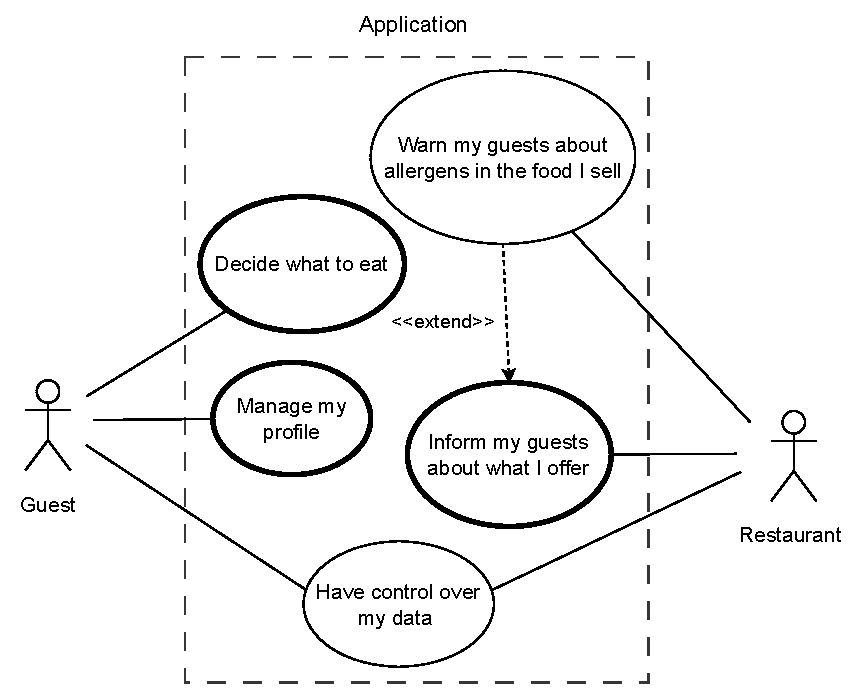
\includegraphics[width=\linewidth]{master-thesis/img/use-cases/use_cases}
  \caption{The application's use case diagram.}
\end{figure}

\newpage

\def\arraystretch{1.5}

\subsection{Guest use cases}
\todo[inline]{change name in figure}
\textbf{UC1: Decide what to order}
\begin{center}
  \begin{tabular}{| l | p{10.75cm} | }
    \hline
    Actor        & Guest \\
    \hline
    Description  & A guest comes to a restaurant and is deciding what to order. \\
    \hline
    Covers & R1.5-R1.9, R1.16 \\
    \hline
    Precondition & The guest has opened a restaurant's menu using the application. \\
    \hline
    Postcondition & The guest is viewing a personalized menu. \\
    \hline
    Scenario     &
    \begin{minipage}[t]{\linewidth}
      \begin{enumerate}[leftmargin=*,nosep,before=\vspace{-0.575\baselineskip},after=\strut]
        \item The guest logs in to the application. \textbf{A1}
        \item The application loads the guest's profile.
        \item The application applies the guest's preferences to the menu.
        \item The application displays the menu enriched with visual clues so that the guest can see what they can and cannot eat.
        \item The guest selects to divide the menu to items they can and items they cannot eat. \textbf{A2 A3}
        \item The application restructures the menu.
      \end{enumerate}
    \end{minipage}
    \\
    \hline
    Alternatives &
    \begin{minipage}[t]{\linewidth}
      \begin{description}[nosep,after=\strut]
        \item [A1:] The guest does not log in. The guest selects what they are allergic to and what diets they follow using controls in the menu. The scenario continues with step 3.
        \item [A2:] The guest selects to sort the menu by whether they can eat an item.
        \item [A3:] The guest selects to filter out items which they cannot eat.
      \end{description}
    \end{minipage}
    \\
    \hline
  \end{tabular}
  \newline
\end{center}

\begin{figure}[h]
  \centering
  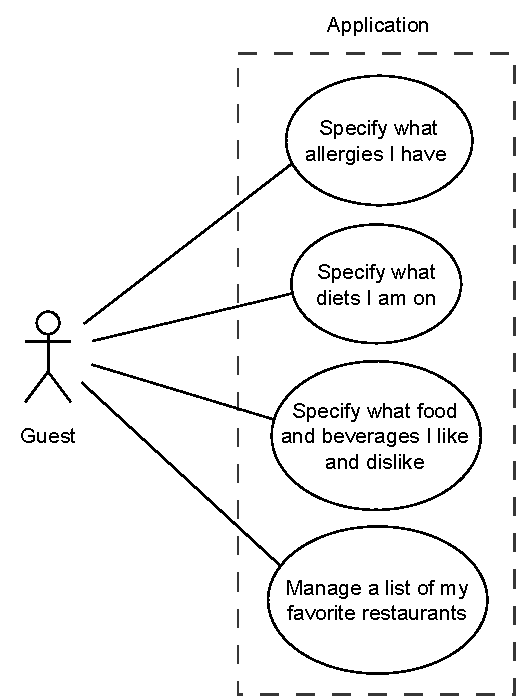
\includegraphics[width=0.62\linewidth]{master-thesis/img/use-cases/use_cases_guest_profile_management}
  \caption{Guest profile management use cases}
\end{figure}

\newpage

\todo[inline]{change name in figure}
\noindent \textbf{UC2: Specify what I am allergic to}
\begin{center}
  \begin{tabular}{| l | p{10.75cm} | }
    \hline
    Actor         & Guest \\
    \hline
    Covers        & R1.1, R1.4 \\
    \hline
    Precondition  & The guest is logged in to the application. \\
    \hline
    Postcondition & The guest's profile contains data about what the guest is allergic to. \\
    \hline
    Scenario      &
    \begin{minipage}[t]{\linewidth}
      \begin{enumerate}[leftmargin=*,nosep,before=\vspace{-0.575\baselineskip},after=\strut]
        \item The guest opens their profile.
        \item The application displays options for what a person can be allergic to.
        \item The guest selects options based on what they are allergic to. \textbf{A1}
        \item The guest presses a button for saving their profile.
        \item The application updates the guest's profile.
      \end{enumerate}
    \end{minipage}
    \\
    \hline
    Alternatives &
    \begin{minipage}[t]{\linewidth}
      \begin{description}[nosep,after=\strut]
        \item [A1:] Some of the options are selected because the guest has already specified them in the past.
      \end{description}
    \end{minipage}
    \\
    \hline
  \end{tabular}
  \newline
\end{center}

\noindent \textbf{UC3: Look up online what a restaurant offers today}
\begin{center}
  \begin{tabular}{| l | p{10.75cm} | }
    \hline
    Actor        & Guest \\
    \hline
    Description  & A guest wants to know what a restaurant serves at the moment. \\
    \hline
    Covers        & R1.10-R1.12, R1.15, R1.16 \\
    \hline
    Scenario     &
    \begin{minipage}[t]{\linewidth}
      \begin{enumerate}[leftmargin=*,nosep,before=\vspace{-0.575\baselineskip},after=\strut]
        \item The guest searches for the restaurant by its name. \textbf{A1 A2 A3 A4}
        \item The application displays the restaurant's detail which contains a list of its menus.
        \item The guest selects a menu.
        \item The application displays the menu. \textbf{A5}         
      \end{enumerate}
    \end{minipage}
    \\
    \hline
    Alternatives &
    \begin{minipage}[t]{\linewidth}
      \begin{description}[nosep,after=\strut] 
        \item [A1:] The guest selects the restaurant in the overview screen from UC4.
        \item [A2:] The guest visits the restaurant's webpage and clicks on a link which takes them to the application.
        \item [A3:] The guest scans a QR code on a printed menu which takes them to the application.
        \item [A4:] The guest specifies the IRI of the restaurant. 
        \item [A5:] The application first translates the menu into the current language of the user interface. 
      \end{description}
    \end{minipage}
    \\
    \hline
  \end{tabular}
  \newline
\end{center}

\newpage

\begin{figure}[h]
  \centering
  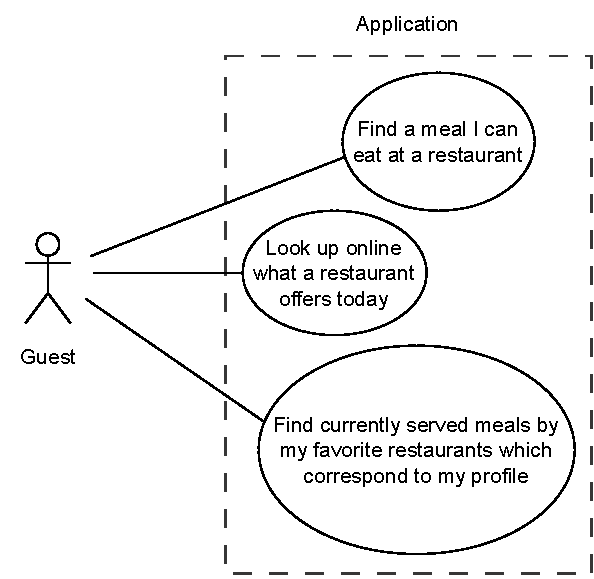
\includegraphics[width=0.62\linewidth]{master-thesis/img/use-cases/use_cases_guest_menu_viewer}
  \caption{Guest menu viewing use cases}
\end{figure}

\todo[inline]{change name in figure}
\noindent \textbf{UC4: See currently served meals by my favorite restaurants which I can eat}
\begin{center}
  \begin{tabular}{| l | p{10.75cm} | }
    \hline
    Actor        & Guest \\
    \hline
    Description  & A guest wants to know what do their favorite restaurants currently offer. \\
    \hline
    Covers & R1.14 \\
    \hline
    Precondition & The guest is logged in to the application. \\
    \hline
    Postcondition & The guest sees an overview of what the guest's favorite restaurants currently serve. \\
    \hline
    Scenario     &
    \begin{minipage}[t]{\linewidth}
      \begin{enumerate}[leftmargin=*,nosep,before=\vspace{-0.575\baselineskip},after=\strut]
        \item The application displays a list of the guest's favorite restaurants with selected items from their menus. \textbf{A1}\textbf{A2} \textbf{A3}
      \end{enumerate}
    \end{minipage}
    \\
    \hline
    Alternatives &
    \begin{minipage}[t]{\linewidth}
      \begin{description}[nosep,after=\strut]
        \item [A1:] The overview is empty because the restaurants do not currently serve anything. The application displays a text with this information.
        \item [A2:] The overview is empty because the guest has not added any favorite restaurants yet. The application displays instructions on how to add a restaurant to the list.
        \item [A2:] One of the favorite restaurants has no valid menu published at the moment. The application displays a text with this information close to the restaurant's name.
      \end{description}
    \end{minipage}
    \\
    \hline
  \end{tabular}
  \newline
\end{center}

\newpage

\noindent \textbf{UC5: Specify what diets I am on}
\begin{center}
  \begin{tabular}{| l | p{10.75cm} | }
    \hline
    Actor       & Guest \\
    \hline
    Covers & R1.2, R1.4 \\
    \hline
    Scenario    &
    \begin{minipage}[t]{\linewidth}
      \begin{enumerate}[leftmargin=*,nosep,before=\vspace{-0.575\baselineskip},after=\strut]
        \item The guest opens their profile.
        \item The application displays a screen with a list of previously specified diets by the guest. \textbf{A1}
        \item The guest presses a button for adding a new diet to the list.
        \item The application displays a search bar.
        \item The guest starts typing the name of a diet into the search bar.
        \item The application suggests diets which contain the given input in their name.
        \item The guest selects the desired diet. \textbf{A2}
        \item The application adds the diet to the guest's profile. \textbf{A3}
        \item The guest repeats steps 3 to 8 until they have specified all of the diets they are on.
      \end{enumerate}
    \end{minipage}
    \\
    \hline
    Alternatives &
    \begin{minipage}[t]{\linewidth}
      \begin{description}[nosep,after=\strut]
        \item [A1:] The list is empty because the guest has not specified any diets yet. The application displays a text containing this information.
        \item [A2:] The application does not recognize the diet which the guest is trying to specify. The guest creates a public issue in the application's repository with a request to add the desired diet to the application.
        \item [A3:] The diet the guest has specified is already contained in the guest's profile. The application informs the guest about this fact and their profile is not altered.
      \end{description}
    \end{minipage}
    \\
    \hline
  \end{tabular}
  \newline
\end{center}

\todo[inline]{add covering of nonfunctional req.}
\noindent \textbf{UC6: Have control over my data}
\begin{center}
  \begin{tabular}{| l | p{10.75cm} | }
    \hline
    Actor        & Guest \\
    \hline
    Description  & A guest wants to specify where should the application store and read their data. \\
    \hline
    Covers & Rx.x \\
    \hline
    Scenario     &
    \begin{minipage}[t]{\linewidth}
      \begin{enumerate}[leftmargin=*,nosep,before=\vspace{-0.575\baselineskip},after=\strut]
        \item The guest navigates to a page for managing data storage options.
        \item The application provides a list of places where it can store data.
        \item The guest selects one of the options.
        \item The application starts using the selected place for storing and reading the guest's data.
      \end{enumerate}
    \end{minipage}
    \\
    \hline
  \end{tabular}
  \newline
\end{center}

\newpage

\noindent \textbf{UC7: Specify what food and beverages I like and dislike}
Covers R1.3, R1.4
\begin{center}
  \begin{tabular}{| l | p{10.75cm} | }
    \hline
    Actor    & Guest \\
    \hline
    Covers & Rx.x \\
    \hline
    Scenario &
    \begin{minipage}[t]{\linewidth}
      \begin{enumerate}[leftmargin=*,nosep,before=\vspace{-0.575\baselineskip},after=\strut]
        \item The guest opens their profile and navigates to a section for managing food preferences.
        \item The application displays a screen with two lists, one containing the foods which the guest likes and the other containing the foods which the guest dislikes. \textbf{A1}
        \item The guest presses a button labeled as "Add food" at the end of the list of foods which they like. \textbf{A2}
        \item The application displays a search bar.
        \item The guest starts typing the name of a food into the search bar.
        \item The application suggests foods which contain the given input text in their name.
        \item The guest selects the desired food and presses an "Add" button. \textbf{A3}
        \item The application adds the specified food to the guest's profile. \textbf{A4}
        \item The guest repeats steps 3 to 8 until they have specified all of their food preferences.
      \end{enumerate}
    \end{minipage}
    \\
    \hline
    Alternatives &
    \begin{minipage}[t]{\linewidth}
      \begin{description}[nosep,after=\strut]
        \item [A1:] Either one or both of the lists are empty because the guest has not specified any of their preferences yet. The application displays a text which informs the guest about this fact.
        \item [A2:] The guest presses a button labeled as "Add food" at the end of the list of foods which they dislike.
        \item [A3:] The application does not recognize the food which the guest is trying to specify. The guest creates a public issue in the application's repository with a request to add the desired food to the application.
        \item [A4:] The guest's profile already contains the specified food. The guest is informed about this fact and their profile is not altered.
      \end{description}
    \end{minipage}
    \\
    \hline
  \end{tabular}
  \newline
\end{center}

\newpage

\todo[inline]{check in other use cases whether I used ',' between A1 and A2}
\noindent \textbf{UC8: Manage a list of my favorite restaurants}
Covers R1.13
\begin{center}
  \begin{tabular}{| l | p{10.75cm} | }
    \hline
    Actor    & Guest \\
    \hline
    Covers & Rx.x \\
    \hline
    Precondition & The guest is logged in to the application. \\
    \hline
    Postcondition & A restaurant is added to the list of the guest's favorite restaurants. \\
    \hline
    Scenario &
    \begin{minipage}[t]{\linewidth}
      \begin{enumerate}[leftmargin=*,nosep,before=\vspace{-0.575\baselineskip},after=\strut]
        
        \item The application displays a list of the guest's favorite restaurants. \textbf{A1 A2}  
        \item The guest presses the button for adding a new restaurant to the list.
        \item The application displays a text input field.
        \item The guest starts typing the name of the restaurant. \textbf{A3}  
        \item The application suggests restaurants which contain the specified text in their name to the user. 
        \item The guest clicks on a restaurant's name. \textbf{A4}
        \item The application adds the selected restaurant to the list. \textbf{A5}
      \end{enumerate}
    \end{minipage}
    \\
    \hline
    Alternatives &
    \begin{minipage}[t]{\linewidth}
      \begin{description}[nosep,after=\strut]
        \item [A1:] The guest is viewing a restaurant's detail. The guest presses the button for marking the restaurant as their favorite. The application adds the restaurant to the guest's profile. \textbf{A1.b}
        \item [A1.b:] The restaurant is already contained in the guest's profile and pressing the button removes the restaurant from it.
        \item [A2:] The list is empty because the guest has not added any restaurants yet. The application displays a text with this information.
        \item [A3:] The guest specifies the restaurant's IRI. \textbf{A3.b}   
        \item [A3.b:] The IRI which the guest specified is not valid. The application informs the guest about this fact and the scenario continues with step 4.
        \item [A4:] The application did not find the desired restaurant because it does not use our application. The application displays a text saying that it was not able to find any restaurants by the specified name. The scenario ends.
        \item [A5:] The guest's profile already contains the restaurant by the specified name. The guest is informed about this fact and their profile is not altered.
      \end{description}
    \end{minipage}
    \\
    \hline
  \end{tabular}
  \newline
\end{center}

\newpage
\subsection{Restaurant use cases}

\noindent \textbf{x. Use case: Create a new menu}
\begin{center}
  \begin{tabular}{| l | p{10.75cm} | }
    \hline
    Actor        & Restaurant \\
    \hline
    Scenario     &
    \begin{minipage}[t]{\linewidth}
      \begin{enumerate}[leftmargin=*,nosep,before=\vspace{-0.575\baselineskip},after=\strut]
        \item The restaurant employee presses a button for creating a new menu.
        \item The application displays a screen with an empty menu. \textbf{A1} \textbf{A2} 
        \item The restaurant employee specifies meta-information about the menu. \textbf{A3}
        \item The restaurant employee specifies the restaurant's contact information. \textbf{A4} \textbf{A5} 
        \todo[inline]{Extension point - all menu options}
        \item The restaurant employee specifies when shall the menu be valid. (Extension point)
        \todo[inline]{Extension point - Warn my guests about allergens in the foods I serve}
        \item The restaurant employee specifies how shall the menu display allergen information. (Extension point) 
        \item The restaurant employee adds categories to the~menu.~\textbf{A6}
        \item The restaurant employee adds individual food items to the menu.
        \item The restaurant employee presses a button for saving the menu.
        \todo[inline]{Extension point - publish, print}
        \item The application saves the menu. \textbf{A7} (Extension point)
      \end{enumerate}
    \end{minipage}
    \\
    \hline
    Alternatives &
    \begin{minipage}[t]{\linewidth}
      \begin{description}[nosep,after=\strut]
        \item [A1:] The restaurant employee selects that they wish to use a template. The application displays a menu with some predefined content.
        \item [A2:] The restaurant employee selects that they wish to create the menu based on an existing menu. The application displays a menu with the contents of the base menu.
        \item [A3:] Meta-information is loaded from the restaurant's profile and inserted to the menu by the application.
        \item [A4:] The restaurant employee does not wish to include the restaurant's contact information in the menu and skips this process. 
        \item [A5:] The application inserts the restaurant's contact information automatically based on the restaurant's profile.
        \item [A6:] The restaurant employee skips the creation of categories.
        \item [A7:] The restaurant employee forgets to specify one of the menu's meta-information options. The application warns the restaurant employee about this fact. The restaurant employee finalizes the creation of the menu and the scenario continues with step 9.
      \end{description}
    \end{minipage}
    \\
    \hline
  \end{tabular}
  \newline
\end{center}

\newpage

\noindent \textbf{x. Use case: Warn my guests about allergens in the foods I serve}
\todo[inline]{add use case number in extends column}
\begin{center}
  \begin{tabular}{| l | p{10.75cm} | }
    \hline
    Actor        & Restaurant \\
    \hline
    Description        & A restaurant employee wants to add information about allergens contained in a menu's items. \\
    \hline
    Extends       &  x: Create a new menu \\
    \hline
    Scenario     &
    \begin{minipage}[t]{\linewidth}
      \begin{enumerate}[leftmargin=*,nosep,before=\vspace{-0.575\baselineskip},after=\strut]
        \item The restaurant employee specifies that numbers shall be used to indicate allergens contained in menu items. \textbf{A1}
        \item The application inserts a predefined allergen table at the end of the menu.
        \item The application later automatically inserts allergens to menu items based on their ingredients.
      \end{enumerate}
    \end{minipage}
    \\
    \hline
    Alternatives &
    \begin{minipage}[t]{\linewidth}
      \begin{description}[nosep,after=\strut]
        \item [A1:] The restaurant employee specifies that allergen labels shall be used in the menu. The scenario continues with step 3.
      \end{description}
    \end{minipage}
    \\
    \hline
  \end{tabular}
  \newline
\end{center}

\noindent \textbf{x. Use case: Create a stable menu}
\begin{center}
  \begin{tabular}{| l | p{10.75cm} | }
    \hline
    Actor        & Restaurant \\
    \hline
    Description  & A restaurant's management wants its restaurant to have a stable menu which will be valid every day of the week. \\
    \hline
    Extends       &  x: Create a new menu \\
    \hline
    Scenario     &
    \begin{minipage}[t]{\linewidth}
      \begin{enumerate}[leftmargin=*,nosep,before=\vspace{-0.575\baselineskip},after=\strut]
        \item The restaurant employee selects that the menu shall be valid every day of the week. \textbf{A1} 
        \item The restaurant employee chooses an option that the menu shall repeat periodically for the selected days.
        \item The restaurant employee specifies that the menu shall be valid all day.
      \end{enumerate}
    \end{minipage}
    \\
    \hline
    Alternatives &
    \begin{minipage}[t]{\linewidth}
      \begin{description}[nosep,after=\strut]
        \item [A1:] The restaurant employee selects the option that the menu will be a stable menu. The application inserts the information about what days of the week shall the menu be valid and when automatically.
      \end{description}
    \end{minipage}
    \\
    \hline
  \end{tabular}
  \newline
\end{center}

\noindent \textbf{x. Use case: Create a stable menu in a foreign language}
\begin{center}
  \begin{tabular}{| l | p{10.75cm} | }
    \hline
    Actor        & Restaurant \\
    \hline
    Description  & A restaurant's management wants its restaurant to have a stable menu written in a foreign language. \\
    \hline
    Extends       &  x: Create a new menu \\
    \hline
    Scenario     &
    \begin{minipage}[t]{\linewidth}
      \begin{enumerate}[leftmargin=*,nosep,before=\vspace{-0.575\baselineskip},after=\strut]
        \item The restaurant employee selects that the menu shall be valid every day of the week. \textbf{A1}
        \item The restaurant employee chooses an option that the menu shall repeat periodically for the selected days.
        \item The restaurant employee specifies that the menu shall be valid all day.
        \item The restaurant employee later adds categories and menu items in the desired language.
      \end{enumerate}
    \end{minipage}
    \\
    \hline
    Alternatives &
    \begin{minipage}[t]{\linewidth}
      \begin{description}[nosep,after=\strut]
        \item [A1:] The restaurant employee selects the option that the menu will be a stable menu. The application inserts the information about what days of the week shall the menu be valid automatically.
      \end{description}
    \end{minipage}
    \\
    \hline
  \end{tabular}
  \newline
\end{center}

\noindent \textbf{x. Use case: Create a list of beverages}
\begin{center}
  \begin{tabular}{| l | p{10.75cm} | }
    \hline
    Actor        & Restaurant \\
    \hline
    Description  &  \\
    \hline
    Extends       &  x: Create a new menu \\
    \hline
    Scenario     &
    \begin{minipage}[t]{\linewidth}
      \begin{enumerate}[leftmargin=*,nosep,before=\vspace{-0.575\baselineskip},after=\strut]
        \item The restaurant employee selects that the menu shall be valid every day of the week. \textbf{A1}
        \item The restaurant employee chooses an option that the menu shall repeat periodically for the selected days. 
        \item The restaurant employee later adds beverages as items of the menu.
      \end{enumerate}
    \end{minipage}
    \\
    \hline
    Alternatives &
    \begin{minipage}[t]{\linewidth}
      \begin{description}[nosep,after=\strut]
        \item [A1:] The restaurant employee selects the option that the menu will be a list of beverages. The application inserts the information about what days of the week shall the menu be valid automatically.
      \end{description}
    \end{minipage}
    \\
    \hline
  \end{tabular}
  \newline
\end{center}

\noindent \textbf{x. Use case: Create a daily menu for tomorrow}
\begin{center}
  \begin{tabular}{| l | p{10.75cm} | }
    \hline
    Actor        & Restaurant \\
    \hline
    Extends       &  x: Create a new menu \\
    \hline
    Scenario     &
    \begin{minipage}[t]{\linewidth}
      \begin{enumerate}[leftmargin=*,nosep,before=\vspace{-0.575\baselineskip},after=\strut]
        \item The restaurant employee specifies the day for which shall the menu be valid.
        \item The restaurant employee continues the process of creating the menu.
      \end{enumerate}
    \end{minipage}
    \\
    \hline
  \end{tabular}
  \newline
\end{center}

\noindent \textbf{x. Use case: Create daily menus for the next week}
\begin{center}
  \begin{tabular}{| l | p{10.75cm} | }
    \hline
    Actor        & Restaurant \\
    \hline
    Extends       &  x: Create a new menu \\
    \hline
    Scenario     &
    \begin{minipage}[t]{\linewidth}
      \begin{enumerate}[leftmargin=*,nosep,before=\vspace{-0.575\baselineskip},after=\strut]
        \item The restaurant employee specifies the day for which shall the menu be valid.
        \item The restaurant employee continues the process of creating the menu.
        \item When the menu is finished, creates the restaurant employee another menu. \textbf{A1}
      \end{enumerate}
    \end{minipage}
    \\
    \hline
    Alternatives &
    \begin{minipage}[t]{\linewidth}
      \begin{description}[nosep,after=\strut]
        \item [A1:] The restaurant employee has created menus for the whole week. The restaurant employee skips this step and the scenario ends.
      \end{description}
    \end{minipage}
    \\
    \hline
  \end{tabular}
  \newline
\end{center}

\begin{figure}[h]
  \centering
  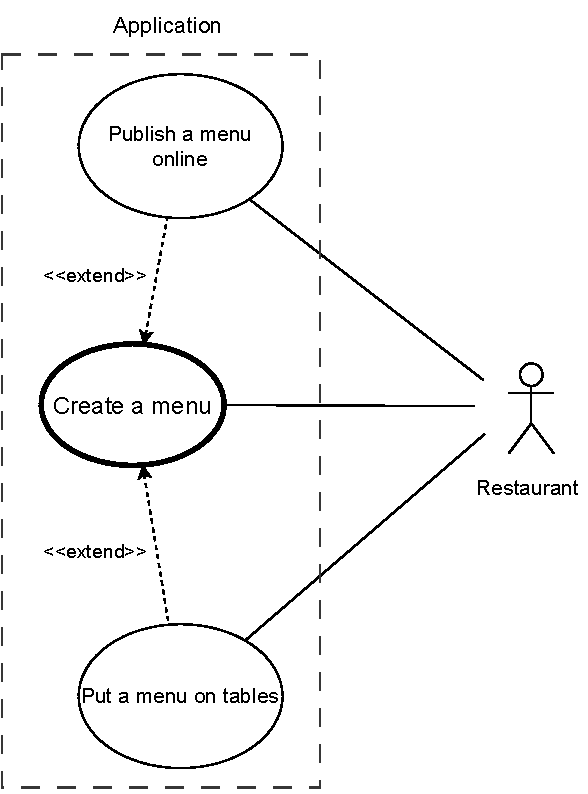
\includegraphics[width=0.62\linewidth]{master-thesis/img/use_cases/use_cases_restaurant_publish_menu}
  \caption{Restaurant offer use cases}
\end{figure}

\begin{figure}[h]
  \centering
  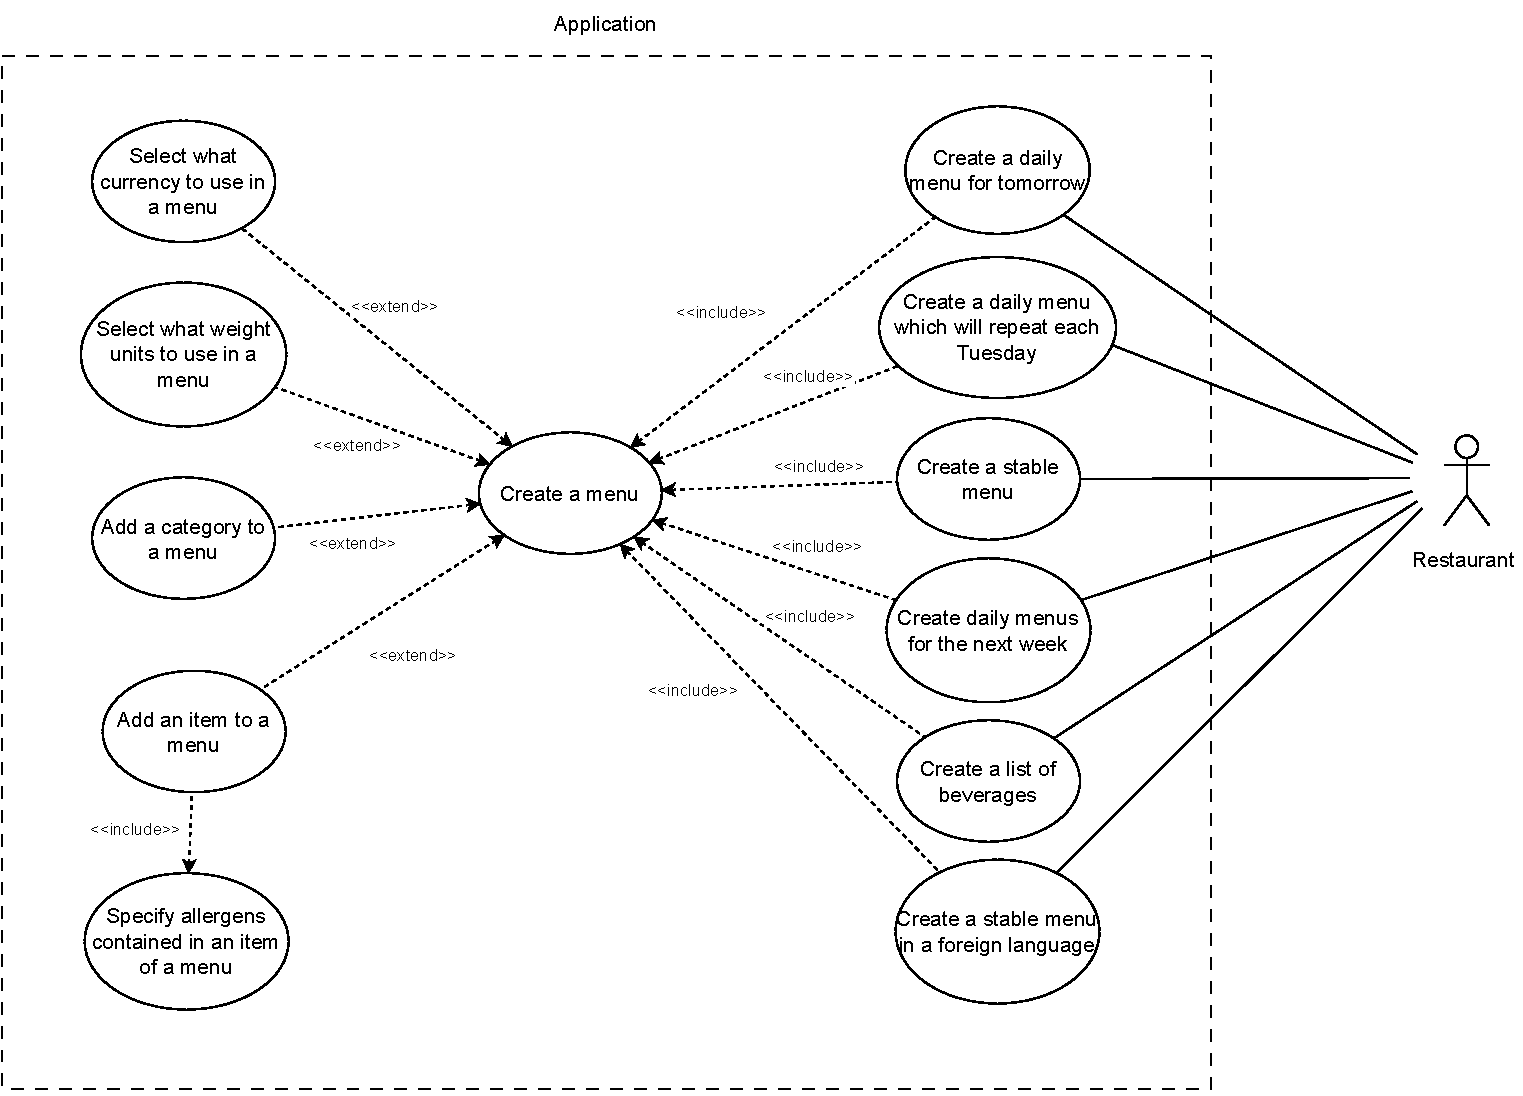
\includegraphics[width=0.62\linewidth]{master-thesis/img/use_cases/use_cases_restaurant_create_menu}
  \caption{Restaurant menu creation use cases}
\end{figure}

\begin{figure}[h]
  \centering
  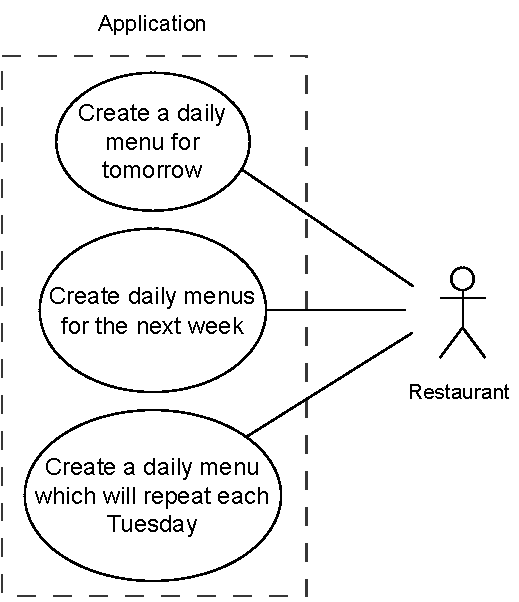
\includegraphics[width=0.62\linewidth]{master-thesis/img/use_cases/use_cases_restaurant_create_daily_menu}
  \caption{Restaurant daily menu creation use cases}
\end{figure}
























% \noindent \textbf{8. Use case: Post a menu online}

% \begin{center}
%   \begin{tabular}{| l | p{10.75cm} | }
%     \hline
%     Actor        & Restaurant \\
%     \hline
%     Description  & A restaurant's management decides to post their currently valid menu online. \\
%     \hline
%     Scenario     &
%     \begin{minipage}[t]{\linewidth}
%       \begin{enumerate}[leftmargin=*,nosep,before=\vspace{-0.575\baselineskip},after=\strut]
%         \item The restaurant employee creates the menu as in the use case x.
%         \item The application generates a URL which points to the application, providing it with the created menu.
%         \item The restaurant employee adds the generated URL to the restaurant's webpage. \textbf{A1}
%       \end{enumerate}
%     \end{minipage}
%     \\
%     \hline
%     Alternatives &
%     \begin{minipage}[t]{\linewidth}
%       \begin{description}[nosep,after=\strut]
%         \item [A1:] The restaurant employee shares the generated URL on the restaurant's social media.
%       \end{description}
%     \end{minipage}
%     \\
%     \hline
%   \end{tabular}
%   \newline
% \end{center}

% \noindent \textbf{9. Use case: Allow my guests to view a menu by scanning a QR code}

% \begin{center}
%   \begin{tabular}{| l | p{10.75cm} |}
%     \hline
%     Actor        & Restaurant \\
%     \hline
%     Description  & A restaurant's management would like to provide a menu with a QR code which will take the restaurant's guests to the application. \\
%     \hline
%     Scenario     &
%     \begin{minipage}[t]{\linewidth}
%       \begin{enumerate}[leftmargin=*,nosep,before=\vspace{-0.575\baselineskip},after=\strut]
%         \item The restaurant employee creates a menu as in use case x, ensuring that a checkbox labeled "Add a QR code" is checked. \textbf{A1}
%         \item The application generates a QR code which will link a guest to the application.
%         \item The restaurant employee prints the menu and puts in on tables as in use case x.
%         \item A guest scans the QR code on the printed menu.
%         \item The application displays the menu.
%       \end{enumerate}
%     \end{minipage}
%     \\
%     \hline
%     Alternatives &
%     \begin{minipage}[t]{\linewidth}
%       \begin{description}[nosep,after=\strut]
%         \item [A1:] The restaurant employee selects a menu from previously created menus.
%       \end{description}
%     \end{minipage}
%     \\
%     \hline
%   \end{tabular}
%   \newline
% \end{center}

% \noindent \textbf{10. Use case: Change an ingredient of a meal in an existing menu}

% \begin{center}
%   \begin{tabular}{| l | p{10.75cm} | }
%     \hline
%     Actor        & Restaurant \\
%     \hline
%     Scenario     &
%     \begin{minipage}[t]{\linewidth}
%       \begin{enumerate}[leftmargin=*,nosep,before=\vspace{-0.575\baselineskip},after=\strut]
%         \item The restaurant employee logs in to the application.
%         \item The restaurant employee clicks an "Edit" button next to a menu.
%         \item The application lets the restaurant employee edit the menu.
%       \end{enumerate}
%     \end{minipage}
%     \\
%     % \hline
%     % Alternatives &
%     % \begin{minipage}[t]{\linewidth}
%     %   \begin{description}[nosep,after=\strut]
%     %     \item [A1:] ...
%     %   \end{description}
%     % \end{minipage}
%     % \\
%     \hline
%   \end{tabular}
%   \newline
% \end{center}

% \noindent \textbf{11. Use case: Place a menu on tables}

% \begin{center}
%   \begin{tabular}{| l | p{10.75cm} | }
%     \hline
%     Actor        & Restaurant \\
%     \hline
%     Description  & A restaurant employee would like to print a menu and place it on tables. \\
%     \hline
%     Scenario     &
%     \begin{minipage}[t]{\linewidth}
%       \begin{enumerate}[leftmargin=*,nosep,before=\vspace{-0.575\baselineskip},after=\strut]
%         \item The restaurant employee logs in to the application.
%         \item The restaurant employee creates a new menu. \textbf{A1}
%         \item The application displays a detail of the menu.
%         \item The restaurant employee clicks a "Print" button in the detail of the menu.
%         \item The application manages to print the menu.
%       \end{enumerate}
%     \end{minipage}
%     \\
%     \hline
%     Alternatives &
%     \begin{minipage}[t]{\linewidth}
%       \begin{description}[nosep,after=\strut]
%         \item [A1:] The restaurant employee selects an existing menu and proceeds with step 3.
%       \end{description}
%     \end{minipage}
%     \\
%     \hline
%   \end{tabular}
%   \newline
% \end{center}

% \noindent \textbf{13. Use case: Reuse an existing daily menu for today.}

% \begin{center}
%   \begin{tabular}{| l | p{10.75cm} | }
%     \hline
%     Actor        & Restaurant \\
%     \hline
%     Description  &  \\
%     \hline
%     Scenario     &
%     \begin{minipage}[t]{\linewidth}
%       \begin{enumerate}[leftmargin=*,nosep,before=\vspace{-0.575\baselineskip},after=\strut]
%         \item The restaurant employee logs in to the application.
%         \item The restaurant employee clicks a button labeled "Create new menu". \textbf{A1}
%         \item The application asks the restaurant employee what kind of menu they would like to create.
%         \item The restaurant employee selects that they wish to create a daily menu.
%         \item The application asks the restaurant employee whether they want to use an existing menu as a template.
%         \item The restaurant employee confirms by clicking a "Yes" button.
%         \item The application displays a list of menus as possible templates.
%         \item The restaurant employee chooses a menu from the list.
%         \item The application loads the chosen menu.
%         \item The restaurant employee changes the date of validity of the menu.
%         \item The restaurant employee clicks a "Save menu" button.
%         \item The application asks the restaurant employee whether they would like to overwrite the existing menu.
%         \item The restaurant employee denies by clicking a "No, create a new menu" button. \textbf{A2}
%         \item The application saves the menu.
%       \end{enumerate}
%     \end{minipage}
%     \\
%     \hline
%     Alternatives &
%     \begin{minipage}[t]{\linewidth}
%       \begin{description}[nosep,after=\strut]
%         \item [A1:] The restaurant employee clicks an "Edit" button next to a menu which they want to reuse. The restaurant employee edits a date field which controls for which day the menu is valid. The restaurant employee then clicks a "Save menu" button and the application saves the menu.
%         \item [A2:] The restaurant employee confirms by clicking a "Yes" button and the application overwrites the old menu with the new one.
%       \end{description}
%     \end{minipage}
%     \\
%     \hline
%   \end{tabular}
%   \newline
% \end{center}

% \begin{figure}[h]
%   \centering
%   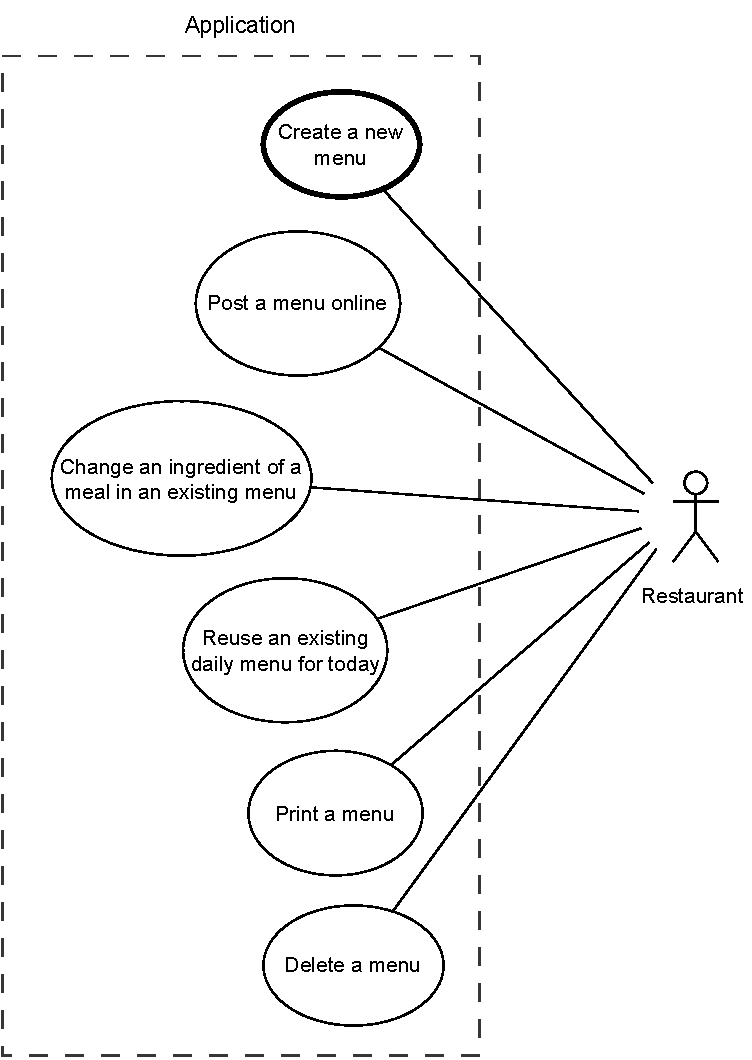
\includegraphics[width=0.62\linewidth]{master-thesis/img/use_cases_restaurant_menu_management}
%   \caption{Restaurant menu creation use cases}
% \end{figure}

% \noindent \textbf{18. Use case: Create a daily menu which will repeat each Tuesday}

% \begin{center}
%   \begin{tabular}{| l | p{10.75cm} | }
%     \hline
%     Actor        & Restaurant \\
%     \hline
%     Description  &  \\
%     \hline
%     Scenario     &
%     \begin{minipage}[t]{\linewidth}
%       \begin{enumerate}[leftmargin=*,nosep,before=\vspace{-0.575\baselineskip},after=\strut]
%         \item The restaurant employee logs in to the application.
%         \item The restaurant employee clicks a button labeled "Create new menu". 
%         \item The application asks the restaurant employee what kind of menu they would like to create.
%         \item The restaurant employee chooses that they wish to create a daily menu.
%         \item The application asks the restaurant employee whether they want to use an existing menu as a template.
%         \item The restaurant employee denies by clicking a "No, create a new menu" button.
%         \item The restaurant employee specifies items of the menu.
%         \item The restaurant employee specifies that the menu will be valid the next Tuesday.
%         \item The restaurant employee ensures that a checkbox labeled "Repeat every week" is checked.
%         \item The restaurant employee clicks a "Save menu" button.
%         \item The application saves the menu.
%       \end{enumerate}
%     \end{minipage}
%     \\
%     \hline
%     % Alternatives &
%     % \begin{minipage}[t]{\linewidth}
%     %   \begin{description}[nosep,after=\strut]
%     %     \item [A1:] 
%     %   \end{description}
%     % \end{minipage}
%     % \\
%     % \hline
%   \end{tabular}
%   \newline
% \end{center}

% \noindent \textbf{x. Use case: Specify where should the application store my data }

% \begin{center}
%   \begin{tabular}{| l | p{10.75cm} | }
%     \hline
%     Actor        & Restaurant \\
%     \hline
%     Description  &  \\
%     \hline
%     Scenario     &
%     \begin{minipage}[t]{\linewidth}
%       \begin{enumerate}[leftmargin=*,nosep,before=\vspace{-0.575\baselineskip},after=\strut]
%         \item ...
%         \item ... \textbf{A1}
%         \item ...
%       \end{enumerate}
%     \end{minipage}
%     \\
%     \hline
%     Alternatives &
%     \begin{minipage}[t]{\linewidth}
%       \begin{description}[nosep,after=\strut]
%         \item [A1:] ...
%       \end{description}
%     \end{minipage}
%     \\
%     \hline
%   \end{tabular}
%   \newline
% \end{center}
\chapter{Existing solutions}
In this chapter we discuss currently available applications which have similar goals to our application.
First we introduce the applications.
After that we form use cases by which we will compare the applications.
Finally, we describe how each application covers the use cases.

\section{Overview of existing applications}
Now we will introduce the currently available applications.

\subsection*{Allergy Menu}
  Allergy menu\footnote{\url{https://allergymenu.uk}  \label{fnlabel}} allows a restaurant employee to maintain a mobile accessible and up-to-date menus that customers can tailor to their food preferences.
  
  A restaurant employee first creates a new menu and adds categories to it, e.g. "Starters" or "Desserts".
  Dishes are then added to each category of the menu.
  A dish contains allergen information as well as flags whether it is suitable for vegans and vegetarians.
  The restaurant employee can also add calories to the dish.

  When a restaurant employee wants to change something in a dish, they can create a copy of the dish which is hidden on the published menu.
  After they finish changes, the dish can be marked as "live", making it appear on the menu with updated content. 

  A dish can optionally contain internal notes, with the ability to upload photographs of products used within the dish.
  The application sends and e-mail regularly to review a menu with all the allergy information.
  An existing menu can be imported to the application in the CSV format.
  Allergy Menu provides an API for food suppliers, allowing them to sync menu information directly into the application without manual intervention.
  
  A guest can interact with a published menu by choosing what allergens they want to avoid.
  The application then filters out items of the menu to meet the guest's preferences.
  A guest can also select an option that they are either a vegan or vegetarian.
  
  A unique restaurant code is used to identify restaurants. 
  This is what guests enter into the application when they want to browse a menu.
  A guest can also find a restaurant which uses the application on a map.

  \newpage

  \begin{figure}[h]
    \centering
    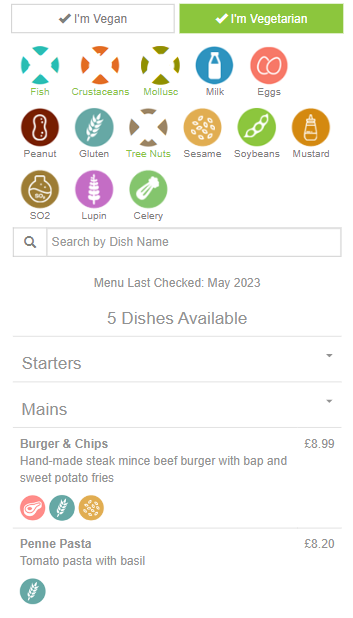
\includegraphics[height=12cm]{master-thesis/img/existing-applications-screenshots/allergy_menu_screenshot}
    \caption{The Allergy Menu application}
  \end{figure}
% end of \subsection

\subsection*{Allergen Checker}
  Allergen Checker\footnote{\url{https://allergenchecker.co.uk/}  \label{fnlabel}} is an allergen management software which enables a restaurant employee to add allergen information to a menu.
  
  A menu is created in three steps.
  In the first step, the restaurant employee creates ingredients which are then stored in a database called the restaurant's "virtual food cupboard".
  During the second step, the restaurant employee creates dishes by specifying their ingredients.
  In the third step, the restaurant employee creates a menu by specifying its dishes.
  
  The application provides a pre-defined list of basic ingredients in its database.
  An ingredient has information about what allergen it contains and also what allergens it may contain. 
  The restaurant employee can also copy information from the ingredient's packaging which will be then displayed in a dish's description in the menu.
  
  Allergen Checker allows for categorizing of dishes and menus. 
  Categories are thought of as a file system for dishes and menus.
  This is convenient when the restaurant employee needs to search for a specific menu or dish.

  \begin{figure}[h]
    \centering
    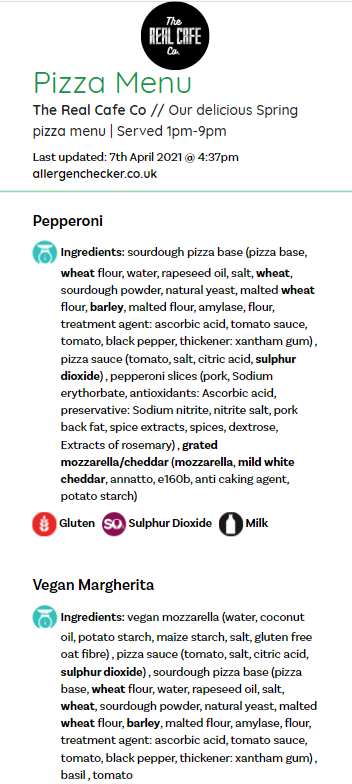
\includegraphics[height=12cm]{master-thesis/img/existing-applications-screenshots/allergen_checker_menu_screenshot}
    \caption{The Allergen Checker application}
  \end{figure}
% end of \subsection

\subsection*{BigZpoon Eagle}
  BigZpoon Eagle\footnote{\url{https://bigzpoon.com/nutrition-menus}  \label{fnlabel}} provides preference-based allergen and nutrition menus for \linebreak restaurants.
  It is a cloud-based SaaS solution which and two parts.

  One part is the consumer-facing website.
  It allows a restaurant's guest to set their dietary restrictions and nutritional goals.
  After this is done, a personalized menu is presented to the guest.
  Items of a menu are shown in three groups.
  There are items which are "Okay to eat", items which are "Okay to eat with modifications" and items which are "Not okay to eat".
  Items and ingredients which are not okay to eat are clearly marked in the item's detail.
  
  The application also supports online ordering of meals.
  The guest can select what they want to eat and choose different ingredients.
  The Eagle platform tries to recommend to the guest what they might want to order using a sort of artificial intelligence algorithm.
  The application also displays detailed nutritional information for the current state of the order and shows whether the guest's nutritional goals are met.

  The consumer-facing website sends analytical data to the backend portal application, which is the other part of the Eagle platform.
  It serves for restaurants to manage their online menus and see insights on how their customers are using the guest application.
  The portal application allows creating multi-location menus to show a different menu based on the restaurant's location.
  The restaurant employee can set up menu groups, categories and individual food items.
  A menu item can be disabled for a certain category, group or restaurant location.
  Creating a menu item involves adding all choices and their variations.
  A restaurant employee can manually create restaurant ingredients or choose from a pre-defined list of ingredients.

  \begin{figure}[h]
    \centering
    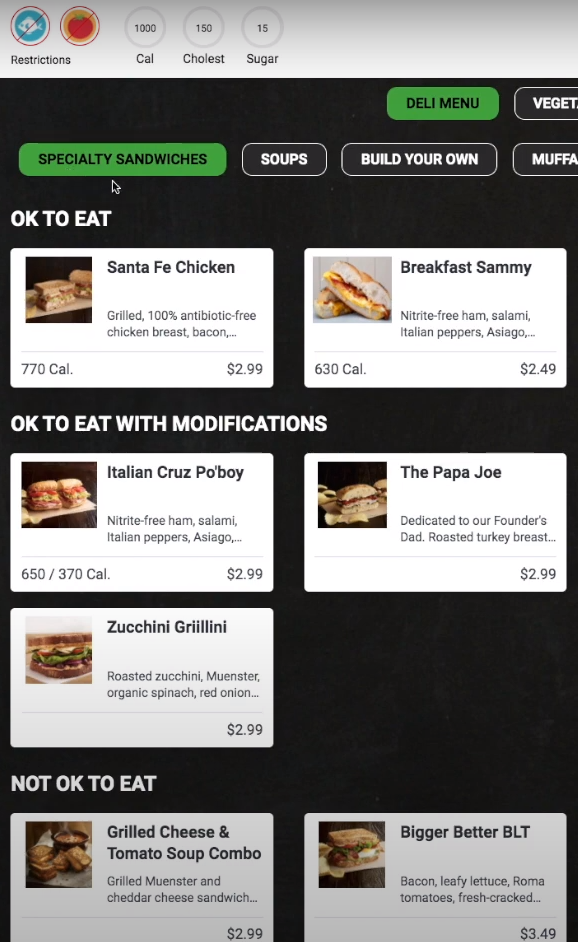
\includegraphics[height=12cm]{master-thesis/img/existing-applications-screenshots/bigzpoon_screenshot}
    \caption{The BigZpoon Eagle application}
  \end{figure}
% end of \subsection

\newpage

\subsection*{Menutech}
  Menutech\footnote{\url{https://menutech.com/en/restaurants}  \label{fnlabel}} provides automated allergen detection, menu translation and design templates for restaurants.
  
  A menu in the application consists of sections and sections contain dishes.
  A restaurant employee can create diets, dishes and recipes.
  A dish can have labels like gluten-free, vegetarian, spicy etc.
  Nutrition rating of a dish can be specified in three levels, from poor to high nutrition.
  A URL linking to more information about the product can be added to a dish.
  The application uses artificial intelligence to suggest items of a menu.
  When specifying allergens, a restaurant employee can copy allergens from existing similar dishes.

  A cover page can be added to a menu.
  A restaurant employee can set colors and font for a menu and the application also provides templates of menus with various styles.
  Translations can be also added to a menu.
  A guest can view a menu as a PDF file or as a mobile friendly version.

  \begin{figure}[h]
    \centering
    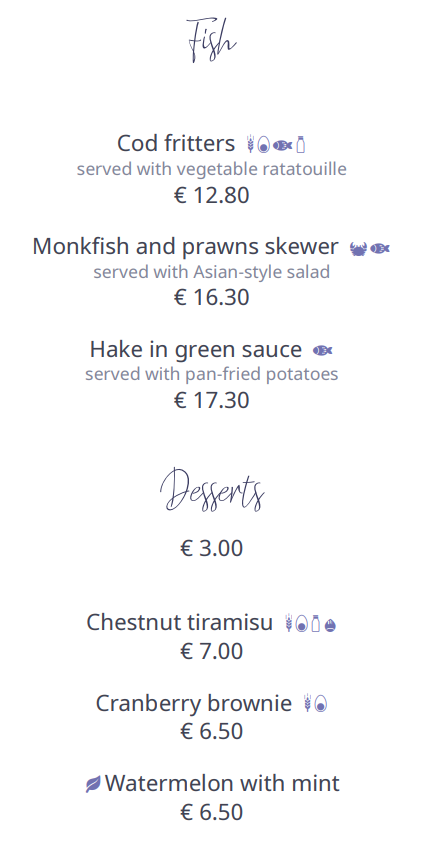
\includegraphics[height=12cm]{master-thesis/img/existing-applications-screenshots/menutech_screenshot}
    \caption{The Menutech application}
  \end{figure}
% end of \subsection

\subsection*{Menu Guide}
  Menu Guide\footnote{\url{https://menuguide.pro/}  \label{fnlabel}} is a tool used to maintain allergen and dietary information, and to share this information with restaurant staff and customers through interactive menus.

  A restaurant employee can create a menu from scratch or an existing menu can be uploaded from a website, pdf, CSV or some other supported formats. 
  A custom message which will be displayed upon opening a menu can be specified.
  The restaurant employee can choose from several menu design templates or apply custom styling using CSS.
  All menus have date of expiration for safety reasons.

  An item of a menu contains information like its name, price, calories and a list of ingredients as plain text.
  The restaurant employee clicks on allergen icons to specify allergens contained in the item.
  An item has more options for how it can contain an allergen. 
  Namely, it can surely contain the allergen, or it may or may not contain the allergen, or it may or may not contain traces of the allergen.
  When ingredients are inserted as text, the application automatically highlights ingredients in the text which contain allergens.
  Some allergens like nuts contain sub-allergens to choose from, e.g. almond or cashew.
  A food item can be marked as vegan, vegetarian or as gluten free etc.
  The restaurant employee can save commonly used menu items into a library for re-use in future. 

  The restaurant employee can create a link between two menus in a parent---child manner.
  When a parent menu is edited, changes are automatically propagated into its child menus.
  Deleting a parent menu will also delete all menus which are linked to it.

  A restaurant guest is able to select allergens and dietary options like being vegan or vegetarian.
  The application can filter or highlight menu items which do not correspond to the guest's selected preferences.
  It can also be set to remember the guest's preferences for future use.

  Menu Guide provides analytical insights like a daily breakdown of page views and the allergens and dietary preferences selected by diners.

  \begin{figure}[h]
    \centering
    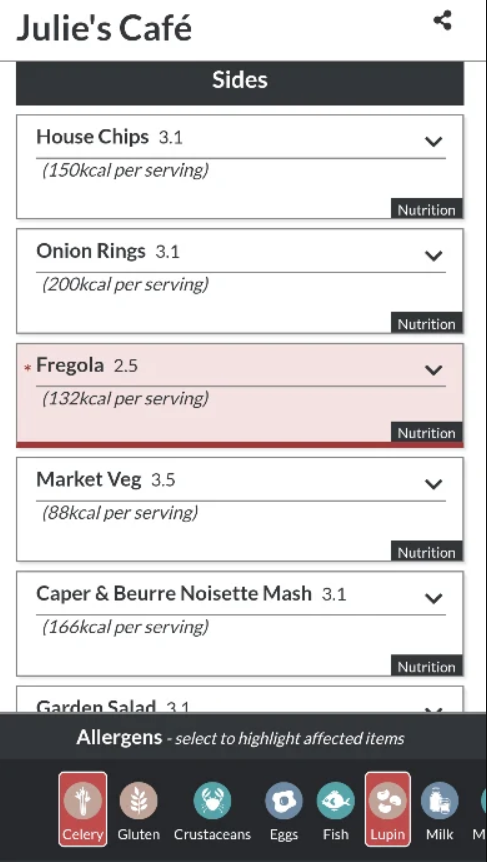
\includegraphics[height=12cm]{master-thesis/img/existing-applications-screenshots/menu_guide_screenshot}
    \caption{The Menu Guide application}
  \end{figure}
% end of \subsection

\section{Comparison of the applications}
First, we are going to specify use cases which an application such as ours should support.
\autoref{comparison-guest-use-cases} contains those use cases in which a guest uses the application.
\autoref{comparison-restaurant-use-cases} then contains those use cases in which a restaurant employee uses the application.

% Guest application use cases
\begin{table}[h]\centering
    \begin{tabular}{| c | l |}
      \hline
      G1 & Display a menu with allergen information. \\
      \hline
      G2 & Highlight items of a menu which the guest cannot eat.  \\
      \hline
      G3 & Hide items of a menu which the guest cannot eat.  \\
      \hline
      G4 & Save the guest's dietary preferences.  \\
      \hline
      G5 & Translate a menu.  \\
      \hline
      G6 & Distinguish whether a menu item is vegan or vegetarian.  \\
      \hline
      G7 & Update the list of the guest's favorite restaurants.  \\
      \hline
      G8 & Let the guest specify where should their data be stored. \\ 
      \hline
    \end{tabular}
    \caption{Application guest use cases}\label{comparison-guest-use-cases}
\end{table}

% Restaurant application use cases
\begin{table}[h]\centering
  \begin{tabular}{| c | l |}
    \hline
    R1 & Add allergen information to a menu. \\
    \hline
    R2 & Save a menu item for future use. \\
    \hline
    R3 & Configure when a menu will be valid. \\
    \hline
    R4 & Provide pre-defined food ingredients. \\
    \hline
    R5 & Have multiple menus of a restaurant active at the same time. \\    
    \hline
    R6 & Generate a QR code for a menu. \\
    \hline 
    R7 & Provide design templates for a new menu. \\
    \hline 
    R8 & Let the restaurant employee specify where to store data. \\
    \hline
  \end{tabular}
  \caption{Application restaurant use cases}\label{comparison-restaurant-use-cases}
\end{table}

\autoref{comparison-guest-use-cases-result} and \autoref{comparison-restaurant-use-cases-result} contain results of the comparison.
Value \ding{52} means that an application supports the given use case.
Value \ding{56} means that an application does not support the given use case. 

% Guest use cases
\begin{table}[h]\centering
  \begin{tabular}{| l | c | c | c | c | c | c | c | c |}
    \hline 
      & G1 & G2 & G3 & G4 & G5 & G6 & G7 & G8 \\
    \hline
    Menutech         & \ding{52} & \ding{56} & \ding{56} & \ding{56} & \ding{52} & \ding{52} & \ding{56} & \ding{56} \\
    \hline
    Allergy Menu     & \ding{52} & \ding{56} & \ding{52} & \ding{56} & \ding{56} & \ding{52} & \ding{56} & \ding{56}  \\
    \hline
    Menu Guide       & \ding{52} & \ding{52} & \ding{52} & \ding{52} & \ding{56} & \ding{52} & \ding{56} & \ding{56}  \\
    \hline
    BigZpoon Eagle   & \ding{52} & \ding{52} & \ding{56} & \ding{56} & \ding{56} & \ding{52} & \ding{56} & \ding{56}  \\
    \hline
    Allergen Checker & \ding{52} & \ding{56} & \ding{56} & \ding{56} & \ding{56} & \ding{56} & \ding{56} & \ding{56}  \\
    \hline
    Choose Well      & \ding{52} & \ding{52} & \ding{52} & \ding{52} & \ding{52} & \ding{52} & \ding{52} & \ding{52} \\
    \hline
  \end{tabular}
  \caption{Comparison of applications regarding use cases with guest}\label{comparison-guest-use-cases-result}
\end{table}

% Restaurant use cases
\begin{table}[h]\centering
  \begin{tabular}{| l | c | c | c | c | c | c | c | c |}
    \hline 
      & R1 & R2 & R3 & R4 & R5 & R6 & R7 & R8 \\
    \hline
    Menutech         & \ding{52} & \ding{52} & \ding{52} & \ding{56} & \ding{52} & \ding{52} & \ding{52} & \ding{56} \\
    \hline
    Allergy Menu     & \ding{52} & \ding{56} & \ding{56} & \ding{56} & \ding{56} & \ding{56} & \ding{56} & \ding{56} \\
    \hline
    Menu Guide       & \ding{52} & \ding{52} & \ding{56} & \ding{56} & \ding{52} & \ding{52} & \ding{52} & \ding{56} \\
    \hline
    BigZpoon Eagle   & \ding{52} & \ding{56} & \ding{52} & \ding{52} & \ding{52} & \ding{56} & \ding{56} & \ding{56} \\
    \hline
    Allergen Checker & \ding{52} & \ding{56} & \ding{52} & \ding{52} & \ding{52} & \ding{56} & \ding{56} & \ding{56} \\
    \hline
    Choose Well      & \ding{52} & \ding{52} & \ding{52} & \ding{52} & \ding{52} & \ding{52} & \ding{56} & \ding{52} \\
    \hline
  \end{tabular}
  \caption{Comparison of applications regarding use cases with restaurant}\label{comparison-restaurant-use-cases-result}
\end{table}

\chapter{Design}
Now we will design how to implement what we have defined in the analysis chapter.
Our application is a single-page web application.

\section{Architecture}
\begin{figure}[h]
  \centering
  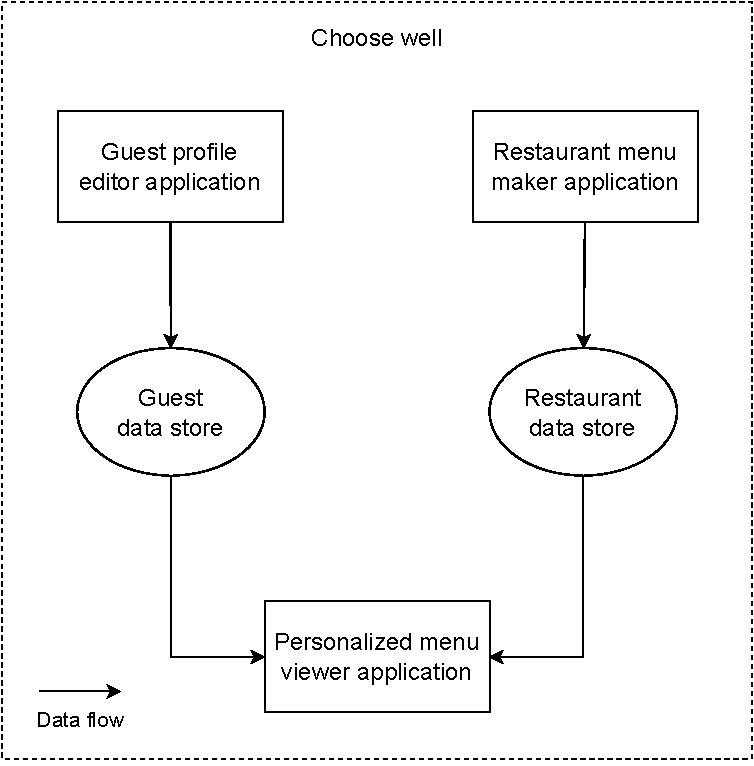
\includegraphics[width=0.62\linewidth]{master-thesis/img/architecture_data_flow.pdf}
  \caption{Application's data flow diagram}
\end{figure}

\todo[inline]{add react router if used}
% \subsection{client-side routing}

\section{Technological stack}
There are various options out there for what technologies we can use to implement our application.
This section contains an overview of available tools and which ones we chose and why.

\subsection{User interface}
  We need a UI so that a user can interact with the application.
  We need to be able to create an interactive user interface.
  We need to have state for logged in user.
  We need to fetch data from the internet.
  We need to integrate with Solid.

  \subsection*{Considered technologies}
  Nowadays, there are many frameworks for building web applications.
  The most popular options are Angular, React and Vue.

  \subsubsection*{Angular}
  Angular is a platform and framework for building single-page client applications using HTML and TypeScript. 
  It implements its core and optional functionality as a set of TypeScript libraries. 
  The basic building blocks of the Angular framework are Angular components that are organized into \emph{NgModules}. 
  NgModules collect related code into functional sets; an Angular application is defined by a set of NgModules.

  \subsubsection*{React.js}
  React is a JavaScript library for rendering user interfaces.
  Applications written in React are built from modular and reusable pieces called components.
  React components receive data and return what should appear on the screen. 
  They can be passed new data in response to an interaction, like when the user types into an input. 
  React will then update the screen to match the new data.
  A notable feature is the use of a virtual Document Object Model, or Virtual DOM. 
  React creates an in-memory data-structure cache, computes the resulting differences on a re-render, and then updates the browser's displayed DOM efficiently. 
  This selective rendering provides a major performance boost.

  \subsubsection*{Vue.js}
  Vue is a JavaScript framework for building user interfaces. 
  It builds on top of standard HTML, CSS, and JavaScript and provides a declarative and component-based programming model.
  Vue uses an HTML-based template syntax that allows programmers to declaratively bind the rendered DOM to the underlying component instance's data.
  Under the hood, Vue compiles the templates into highly-optimized JavaScript code. 
  Combined with the reactivity system, Vue can intelligently figure out the minimal number of components to re-render and apply the minimal amount of DOM manipulations when the app state changes.

  \subsection*{Chosen technology}
  We decide to choose \textbf{React} for developing the UI of our application.
  One of the reasons for this decision is that Solid is written for React.
  There exists a Solid React SDK which can help us to work with some of the core Solid principles.
  Ract also allows us to work with components as functions.
% end of \subsection

\subsection{Programming language}
  We need to implement the application.

  \subsection*{Considered technologies}
  As for programming languages, we considered two options. 
  JS, TS

  \subsubsection*{JavaScript}
  JavaScript is a lightweight, interpreted, or just-in-time compiled programming language with first-class functions. 
  It is most well-known as the scripting language for Web pages. 
  JavaScript is a prototype-based, multi-paradigm, single-threaded, dynamic language, supporting object-oriented, imperative, and declarative---e.g. functional programming styles.

  \subsubsection*{TypeScript}
  TypeScript is a superset of JavaScript. 
  It provides features such as optional static typing, classes, interfaces, and generics. 
  The goal of TypeScript is to help catch mistakes early through its type system and make JavaScript development more efficient. 
  One of the big benefits is enabling IDEs to provide a richer environment for spotting common errors as the programmer types their code.

  \subsection*{Chosen technology}
  The goal is to make as few bugs during development as possible and that is why we decide to go with \textbf{Typescript}.
  Defining types of variables makes the code more readable to other developers.
% end of \subsection

\subsection{Build tool}

  \subsection*{Considered technologies}

  \subsubsection*{Vite}
  Vite (French: [vit], like "veet") is a local development server written by Evan You and used by default by the Vue project templates. It has support for TypeScript and JSX.

  It monitors files as they're being edited and upon file save the web browser reloads the code being edited through a process called Hot Module Replacement (HMR) which works by just reloading the specific file being changed using ES6 modules (ESM) instead of recompiling the entire application.

  Vite is a newer build tool that has gained popularity in recent years. It was created to address the limitations of existing build tools, particularly in the development phase. Vite is a build tool that is optimized for speed. It leverages the latest browser technologies, such as ES modules and native browser imports, to provide fast build times.

  Vite is particularly useful for small to medium-sized projects that do not require complex configurations. It is built on top of the Rollup bundler, which is known for its fast build times. Vite also provides a development server that is optimized for performance. The server leverages HTTP/2 server push, which enables the server to send multiple responses for a single client request.

  \subsubsection*{Create React App}
  Create React App is built on Webpack and Babel and it is a popular tool that enables developers to quickly set up a React project. It is an officially supported tool by the React team, making it a reliable choice. It creates a basic React application with all the necessary configuration files, dependencies, and scripts. The tool provides a pre-configured environment that abstracts away much of the configuration that developers would typically have to handle manually. This means that the developer can focus on writing code rather than configuration files.

  \subsection*{Chosen technology}

% end of \subsection


\subsection{nasadenie}
% GH Pages


\subsection{Package manager}
  We need a tool to manage our application's dependencies.
  A package manager can seamlessly handle installing and uninstalling of packages which is another name for JavaScript libraries.

  \subsection*{Considered technologies}
  For package management in our application we consider two options: npm and yarn.

  \subsubsection*{npm}
  npm is a package manager for the JavaScript programming language.
  npm is used to fetch any packages that an application needs for development, testing, and/or production, and may also be used to run tests and tools used in the development process.
  It consists of a command line client, also called npm, and an online database of packages, called the npm registry. 
  The registry is accessed via the client, and the available packages can be browsed and searched via the npm website.

  \subsubsection*{yarn}
  A successful and popular alternative package manager is Yarn. 
  Yarn resolves the dependencies using a different algorithm that can mean a faster user experience.
  More specifically, yarn can download packages in parallel to maximize network utilization.

  \subsection*{Chosen technology}
  Although Yarn is just as good as npm for handling packages, the latter is more widely used.
  For this reason we decide to use \textbf{npm} for our application. 
% end of \subsection

\subsection{Responsive design}
  Responsive web design or RWD is a web design approach to make web pages render well on all screen sizes and resolutions while ensuring good usability.
  We need our application to be responsive to various device screens.
  We want a mobile-first approach as most people use smartphones these days.
  The chosen tool should be well documented for ease of use.

  \subsection*{Considered technologies}
  Two options were considered, which are Bootstrap, Material UI.
  Let us briefly introduce them.

  \subsubsection*{Bootstrap}
  Made by myself and Jacob Thornton, Bootstrap is an open-source front-end toolkit created to help designers and developers quickly and efficiently build awesome stuff online. Our goal is to provide a refined, well-documented, and extensive library of flexible design components built with HTML, CSS, and JavaScript for others to build and innovate on.

  The most prominent components of Bootstrap are its layout components, as they affect an entire web page. The basic layout component is called "Container", as every other element in the page is placed in it.

  Once a container is in place, other Bootstrap layout components implement a CSS Flexbox layout through defining rows and columns.

  \subsubsection*{Material Design}
  Material Design is a design language which uses grid-based layouts, responsive animations and transitions, padding, and depth effects such as lighting and shadows.

  The main purpose of Material Design is the creation of a visual language that combines principles of good design with technical and scientific innovation. 

  Designers optimize users' experience with 3D effects, realistic lighting and animation features in immersive, platform-consistent GUIs.

  \subsection*{Chosen technology}

% end of \subsection

\subsection{Persistence}
We need to store and later read data.
% Solid pods

\subsection{Testing}
% napisat ze som si vybral tu a tu kniznicu 
We need to test our application in order to prevent bugs during implementation.
% https://legacy.reactjs.org/docs/testing-environments.html
\subsection*{Considered technologies}

\subsubsection*{}

\subsubsection*{}

\subsection*{Chosen technology}

\subsection{Documentation}
We need to capture how our application works for users and future developers.
% (GitHub markdown)


\subsection{Authentication}
% inrupt solid-client
\chapter{Implementation}
login.inrupt.com - profile is defaultly not publicly accessible - you need to configure rights to read the dataset in pod browser - shouldn't be profile public by default?
\chapter{Documentation}
\section{User documentation}
\section{Programmer documentation}
\section{Administrator documentation}
\chapter{Testing}
\section{Unit tests}
\section{Performance tests}
\section{End user tests}
\subsection{System Usability Scale}
% \section{Wireframes}
Let's now look at what the users of our application will see.
\todo[inline]{add figure numbers}
Figure x contains a mockup of the guest profile editor application.
On the screen, the guest can see what their dietary profile currently contains.
There are controls for adding information to the profile and for saving it.

\begin{figure}[h]
  \centering
  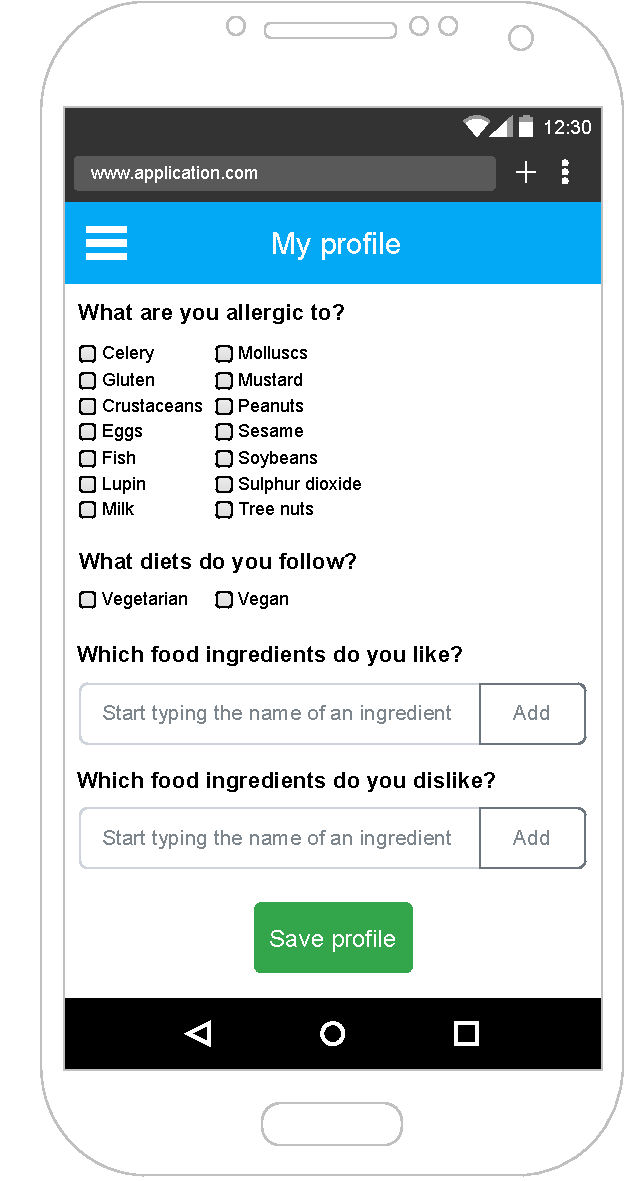
\includegraphics[width=0.62\linewidth]{master-thesis/img/wireframes/dietary_profile_editor.pdf}
  \caption{The guest profile editor application}
\end{figure}

Figure x shows what will the restaurant employee see when they log in to the restaurant menu maker application.
The screen contains a list of previously created menus by the restaurant employee.
Each menu has buttons to view, edit and delete the menu.
There is also a button for creating a new menu.

\begin{figure}[h]
  \centering
  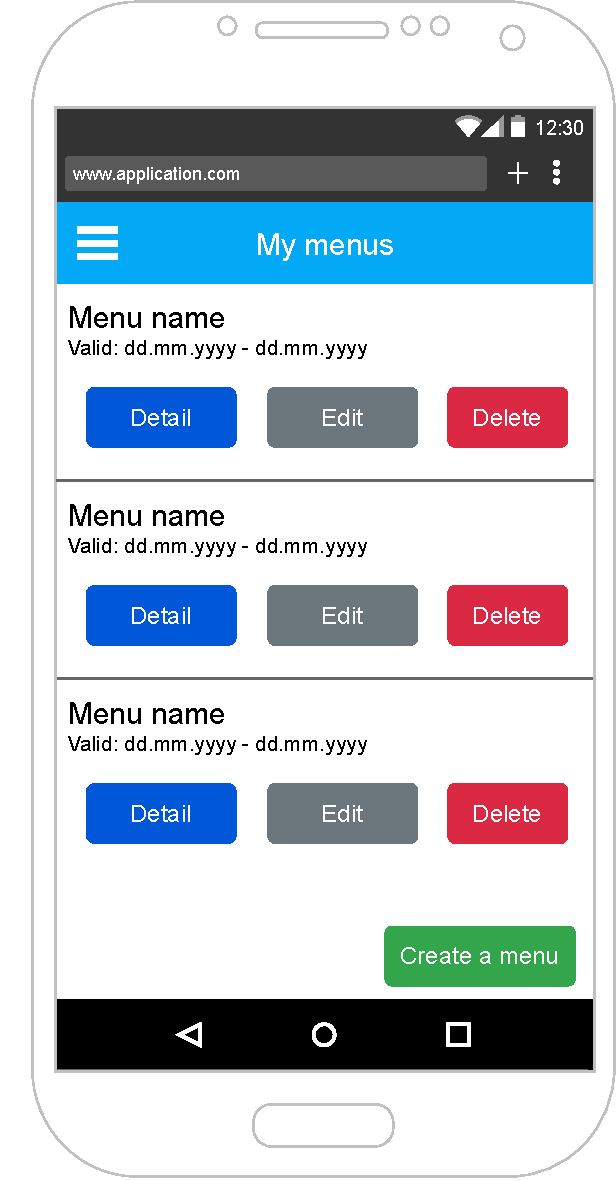
\includegraphics[width=0.62\linewidth]{master-thesis/img/wireframes/menu_creator_menus_overview.pdf}
  \caption{The menus overview screen of the restaurant menu maker application}
\end{figure}

Figure x contains a mockup of the screen which is displayed when a restaurant employee is creating a new menu.
There are fields for specifying the menu's name and date of validity.
There are also buttons for adding either an existing item or a new item to the menu.

\todo[inline]{add categories to menus}
\begin{figure}[h]
  \centering
  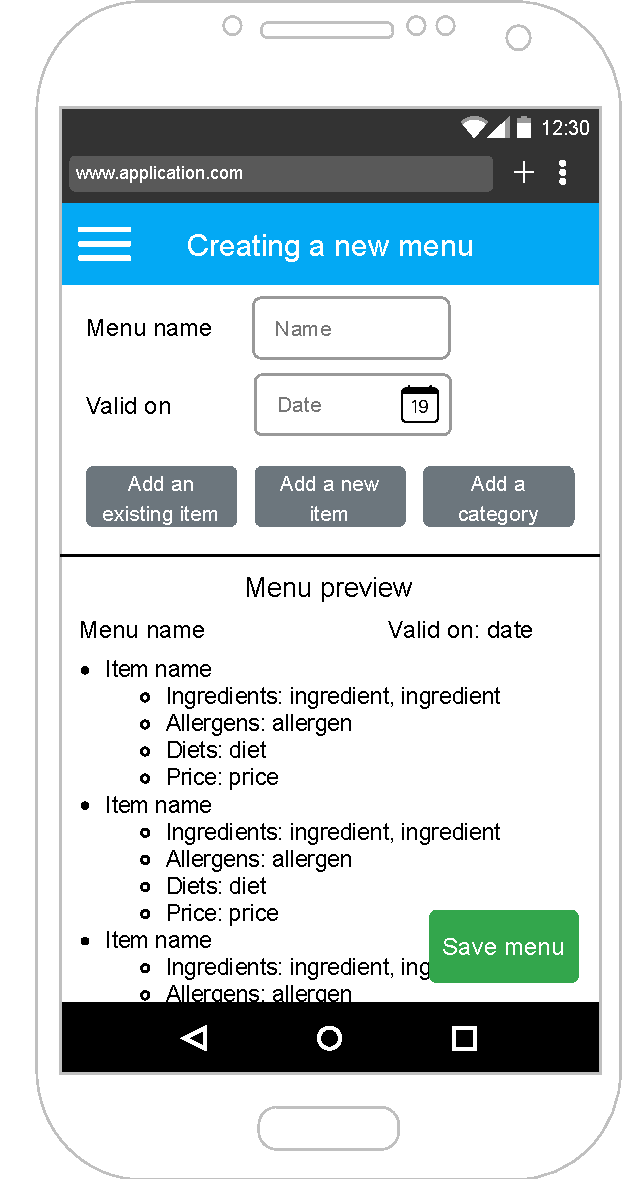
\includegraphics[width=0.62\linewidth]{master-thesis/img/wireframes/menu_creator_new_menu.pdf}
  \caption{The new menu screen of the restaurant menu maker application}
\end{figure}

Figure x shows a screen which is displayed when a restaurant guest logs in to the personalized menu viewer application.
\todo[inline]{remove buttons next to restaurant names}
The screen contains an overview of currently served foods by the guest's favorite restaurants.
A restaurant's name is a clickable link which takes the guest to the restaurant's detail.

\begin{figure}[h]
  \centering
  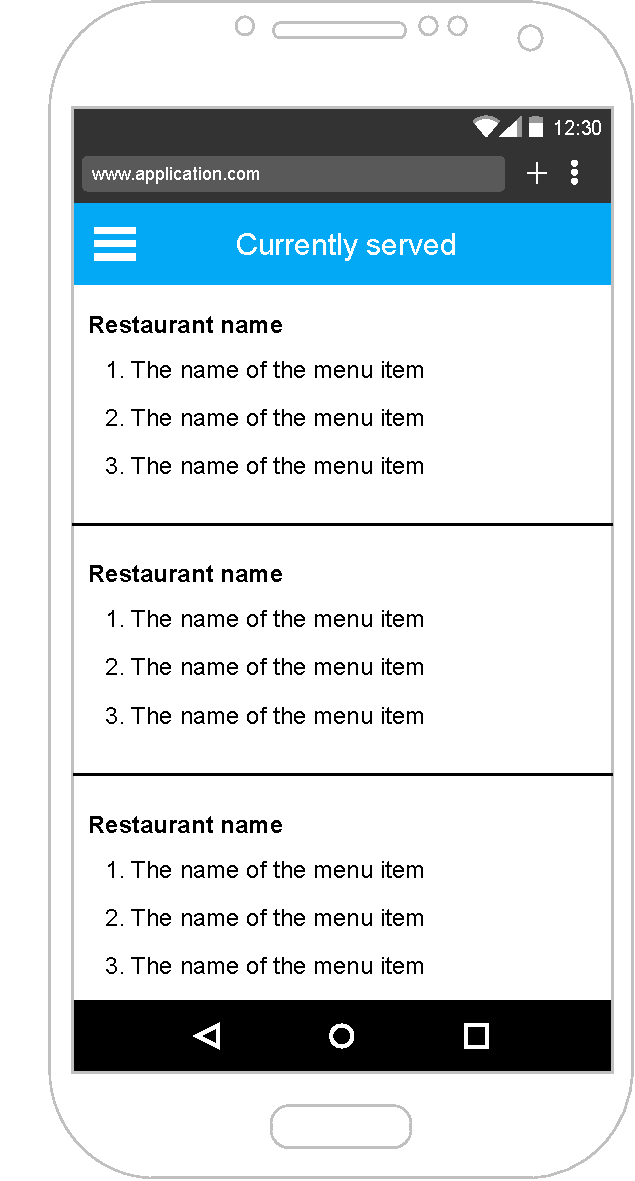
\includegraphics[width=0.62\linewidth]{master-thesis/img/wireframes/menu-viewer-currently-served.pdf}
  \caption{The personalized menu viewer application's home page}
\end{figure}

A detail of a menu can be seen in the figure x.
The menu is divided into two sections.
The first section contains the items which the guest can eat.
The second section contains the items which the guest cannot eat and within each item, the reason why the guest should avoid the food is highlighted, e.g. that it contains a certain allergen which the guest is allergic to.

\begin{figure}[h]
  \centering
  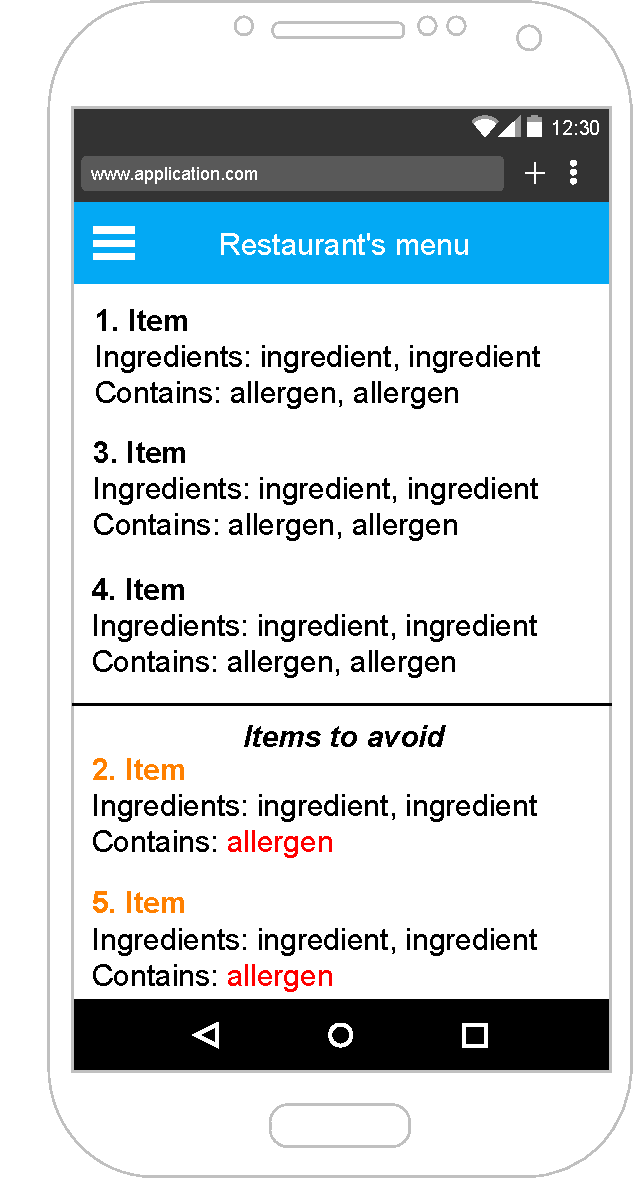
\includegraphics[width=0.62\linewidth]{master-thesis/img/wireframes/menu_viewer_menu_detail.pdf}
  \caption{The personalized menu viewer application's menu detail}
\end{figure}

% \section{Ontology}
Choose Well defines its own RDF vocabulary. 
% \todo[inline]{add figure number}
Fig. x contains the created ontology as a UML class diagram. 
The diagram uses these prefixes:
% \todo[inline]{change font of prefixes to code}
% \todo[inline]{add arrow symbols for prefixes}
% \todo[inline]{add hashtags: /blob/main/choosewellHASHTAG http://www.w3.org/2000/01/rdf-schemaHASHTAG}
\begin{itemize}[noitemsep,nolistsep]
  \item cw: https://github.com/JiriResler/solid-choose-well-ontology/ \newline blob/main/choosewell for the Choose Well ontology.
  \item schema: \textbf{http://schema.org/} for the Schema.org general vocabulary. 
  \item rdfs: \textbf{http://www.w3.org/2000/01/rdf-schema} for the RDF Schema which provides a data-modelling vocabulary for RDF data.
  \item wikidata: \textbf{http://www.wikidata.org/entity/} for describing entities using the Wikidata knowledge base.
\end{itemize}

\begin{figure}[h]
  \centering
  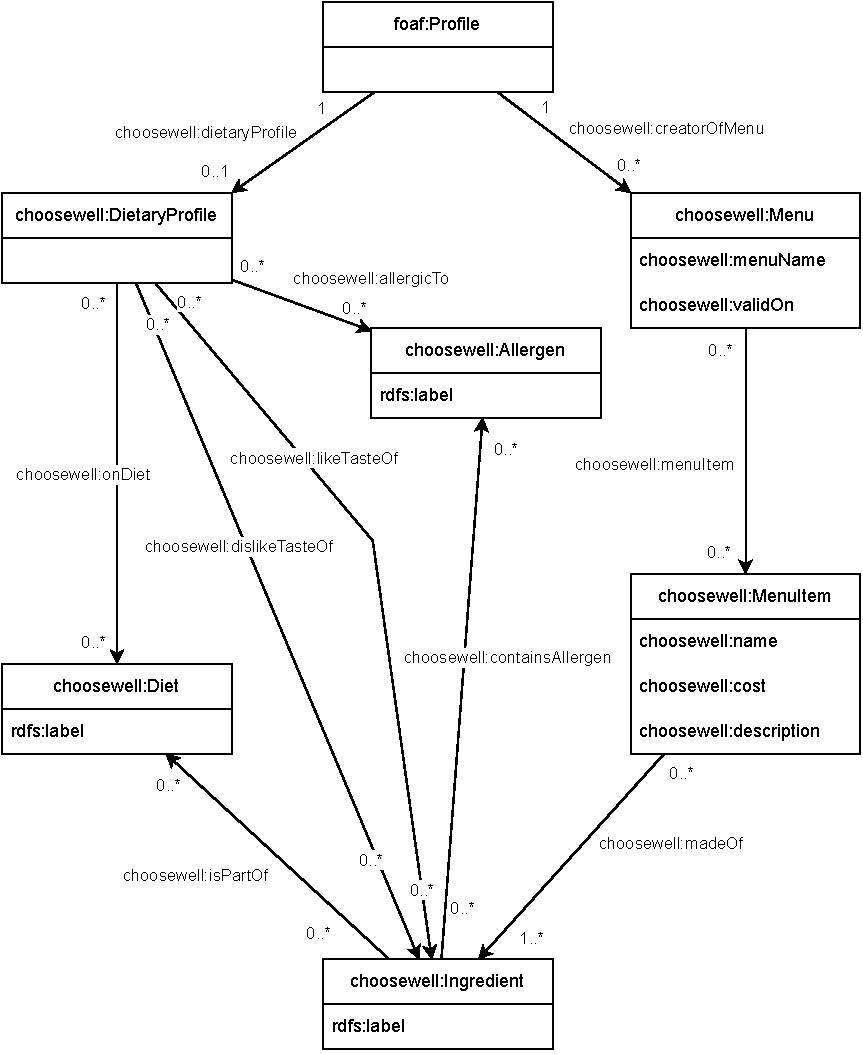
\includegraphics[width=\linewidth]{master-thesis/img/design-ontology.pdf}
  \caption{Ontology}
\end{figure}
\chapter*{Conclusion}
\addcontentsline{toc}{chapter}{Conclusion}

%%% Bibliography
%%% Bibliography (literature used as a source)
%%%
%%% We employ bibTeX to construct the bibliography. It processes
%%% citations in the text (e.g., the \cite{...} macro) and looks up
%%% relevant entries in the bibliography.bib file.
%%%
%%% The \bibliographystyle command selects, which style will be used
%%% for references from the text. The argument in curly brackets is
%%% the name of the corresponding style file (*.bst). Both styles
%%% mentioned in this template are included in LaTeX distributions.

\bibliographystyle{plainnat}    %% Author (year)
% \bibliographystyle{unsrt}     %% [number]

\renewcommand{\bibname}{Bibliography}

%%% Generate the bibliography. Beware that if you cited no works,
%%% the empty list will be omitted completely.

\bibliography{bibliography}

%%% If case you prefer to write the bibliography manually (without bibTeX),
%%% you can use the following. Please follow the ISO 690 standard and
%%% citation conventions of your field of research.

% \begin{thebibliography}{99}
%
% \bibitem{lamport94}
%   {\sc Lamport,} Leslie.
%   \emph{\LaTeX: A Document Preparation System}.
%   2nd edition.
%   Massachusetts: Addison Wesley, 1994.
%   ISBN 0-201-52983-1.
%
% \end{thebibliography}

%%% Figures used in the thesis
\listoffigures
%%% Tables used in the thesis 
\listoftables
%%% Abbreviations used in the thesis, if any, including their explanation
\chapwithtoc{List of Abbreviations}
EU - European Union
UI - user interface
IRI
URL
RDF
CSV
API
SaaS
AI
QR
pdf
W3C
SQL
SPARQL
SDK

Glossary - nezname pojmy
Linked Data
Solid pod
WebID
Solid provider
RDF vocabulary

%%% Attachments to the master thesis, if any. Each attachment must be
%%% referred to at least once from the text of the thesis. Attachments
%%% are numbered.
%%%
%%% The printed version should preferably contain attachments, which can be
%%% read (additional tables and charts, supplementary text, examples of
%%% program output, etc.). The electronic version is more suited for attachments
%%% which will likely be used in an electronic form rather than read (program
%%% source code, data files, interactive charts, etc.). Electronic attachments
%%% should be uploaded to SIS and optionally also included in the thesis on a~CD/DVD.
%%% Allowed file formats are specified in provision of the rector no. 72/2017.
\appendix
\chapter{Attachments}

\section{First Attachment}

\openright
\end{document}
